%%%%%%%%%%%%%%%%%%%%%%%%%%%%%%%%%%%%%%%%%%%%%%%%%%
% Basic setup. Most papers should leave these options alone.
\documentclass[fleqn,usenatbib]{mnras}

% MNRAS is set in Times font. If you don't have this installed (most LaTeX
% installations will be fine) or prefer the old Computer Modern fonts, comment
% out the following line
%\usepackage{newtxtext,newtxmath}
% Depending on your LaTeX fonts installation, you might get better results with one of these:
%\usepackage{mathptmx}
%\usepackage{txfonts}
% 
% Use vector fonts, so it zooms properly in on-screen viewing software
% Don't change these lines unless you know what you are doing
% \usepackage[T1]{fontenc}

% Allow "Thomas van Noord" and "Simon de Laguarde" and alike to be sorted by "N" and "L" etc. in the bibliography.
% Write the name in the bibliography as "\VAN{Noord}{Van}{van} Noord, Thomas"
\DeclareRobustCommand{\VAN}[3]{#2}
\let\VANthebibliography\thebibliography
\def\thebibliography{\DeclareRobustCommand{\VAN}[3]{##3}\VANthebibliography}


%%%%% AUTHORS - PLACE YOUR OWN PACKAGES HERE %%%%%

% Only include extra packages if you really need them. Common packages are:
\usepackage{graphicx}	% Including figure files
\usepackage{amsmath}	% Advanced maths commands
\usepackage{amssymb}	% Extra maths symbols

%%%%%%%%%%%%%%%%%%%%%%%%%%%%%%%%%%%%%%%%%%%%%%%%%%

%%%%% AUTHORS - PLACE YOUR OWN COMMANDS HERE %%%%%

\newcommand{\tcools}{t_{10^5\,{\rm K}}}
\newcommand{\Mdot}{\dot{M}}
\newcommand{\Rvir}{r_{\rm vir}}
\newcommand{\nH}{n_{\rm H}}
\newcommand{\Tvir}{T_{\rm vir}}
\newcommand{\msun}{{\rm M}_\odot}
\newcommand{\vvir}{v_{\rm vir}}
\newcommand{\Nsample}{17}

%%%%%%%%%%%%%%%%%%%%%%%%%%%%%%%%%%%%%%%%%%%%%%%%%%

%%%%%%%%%%%%%%%%%%% TITLE PAGE %%%%%%%%%%%%%%%%%%%

\title[Rotating cooling flows and thin galactic discs]{Hot-mode accretion and the physics of thin-disc~galaxy~formation}

% The list of authors, and the short list which is used in the headers.
% If you need two or more lines of authors, add an extra line using \newauthor
\author[Hafen, Stern, Bullock et al.]{
Zachary Hafen$^{1,2}$\thanks{E-mail: zhafen@uci.edu},
Jonathan Stern$^{2,3}$,
James Bullock$^{1}$,
\ldots
\\
% List of institutions
$^1$ Department of Physics and Astronomy, University of California Irvine, CA 92697, USA \\
$^2$ Department of Physics \& Astronomy and CIERA, Northwestern University, 1800 Sherman Ave, Evanston, IL 60201, USA \\
$^3$ School of Physics \& Astronomy, Tel Aviv University, Tel Aviv 69978, Israel
}

% These dates will be filled out by the publisher
\date{Accepted XXX. Received YYY; in original form ZZZ}

% Enter the current year, for the copyright statements etc.
\pubyear{2020}

% Don't change these lines

\begin{document}
\label{firstpage}
\pagerange{\pageref{firstpage}--\pageref{lastpage}}
\maketitle

% Abstract of the paper
\begin{abstract}
We use FIRE simulations to study disc formation in $z\sim 0$, Milky Way-mass galaxies, and conclude that a key ingredient for the formation of thin stellar discs is the ability for accreting gas to internally exchange angular momentum and develop a narrow and closely-aligned angular momentum distribution prior to joining the galaxy.
Among galaxies with a high fraction of young stars ($>70\%$) in a thin disc ($h/R \sim 0.1$) we find that:
(i) hot, virial-temperature gas dominates the inflowing gas mass on halo scales ($\gtrsim 20$ kpc), with radiative losses offset by compression heating;
(ii) this hot accretion proceeds until angular momentum support stalls inward motion, at which point the gas cools to $\lesssim10^4\,{\rm K}$; 
(iii) concurrent with cooling, the accreting gas transitions from a hot, quasi-spherical configuration to a cool, flattened, disc-like configuration, with a coherent angular momentum distribution aligned with the galaxy disc.
We further show that the existence of this ``rotating cooling flow'' accretion mode is strongly correlated with the fraction of stars forming in a thin disc, among a sample of \Nsample\ $z\sim0$ galaxies spanning a halo mass range of $10^{10.5} M_\odot \lesssim M_{\rm h} \lesssim 10^{12} M_\odot$, or $10^8 M_\odot \lesssim M_\star \lesssim 10^11 M_\odot$.
Notably, galaxies with a thick disc or irregular morphology do not have angular momentum alignment of gas prior to accretion and show no correspondence between halo gas cooling and flattening.
Our results suggest that rotating cooling flows (or, more generally, rotating subsonic flows) that become coherent and angular momentum-supported prior to direct deposition onto the galaxy are likely a necessary condition for the formation of thin, star-forming disc galaxies in a $\Lambda$CDM universe.
\end{abstract}

% Select between one and six entries from the list of approved keywords.
% Don't make up new ones.
\begin{keywords}
galaxies: disc -- galaxies: evolution -- galaxies: haloes -- cosmology: theory
\end{keywords}

%%%%%%%%%%%%%%%%%%%%%%%%%%%%%%%%%%%%%%%%%%%%%%%%%%

%%%%%%%%%%%%%%%%% BODY OF PAPER %%%%%%%%%%%%%%%%%%

\section{Introduction}
\label{s: introduction}

% THE THIN DISCS
\begin{figure*}
    \centering
    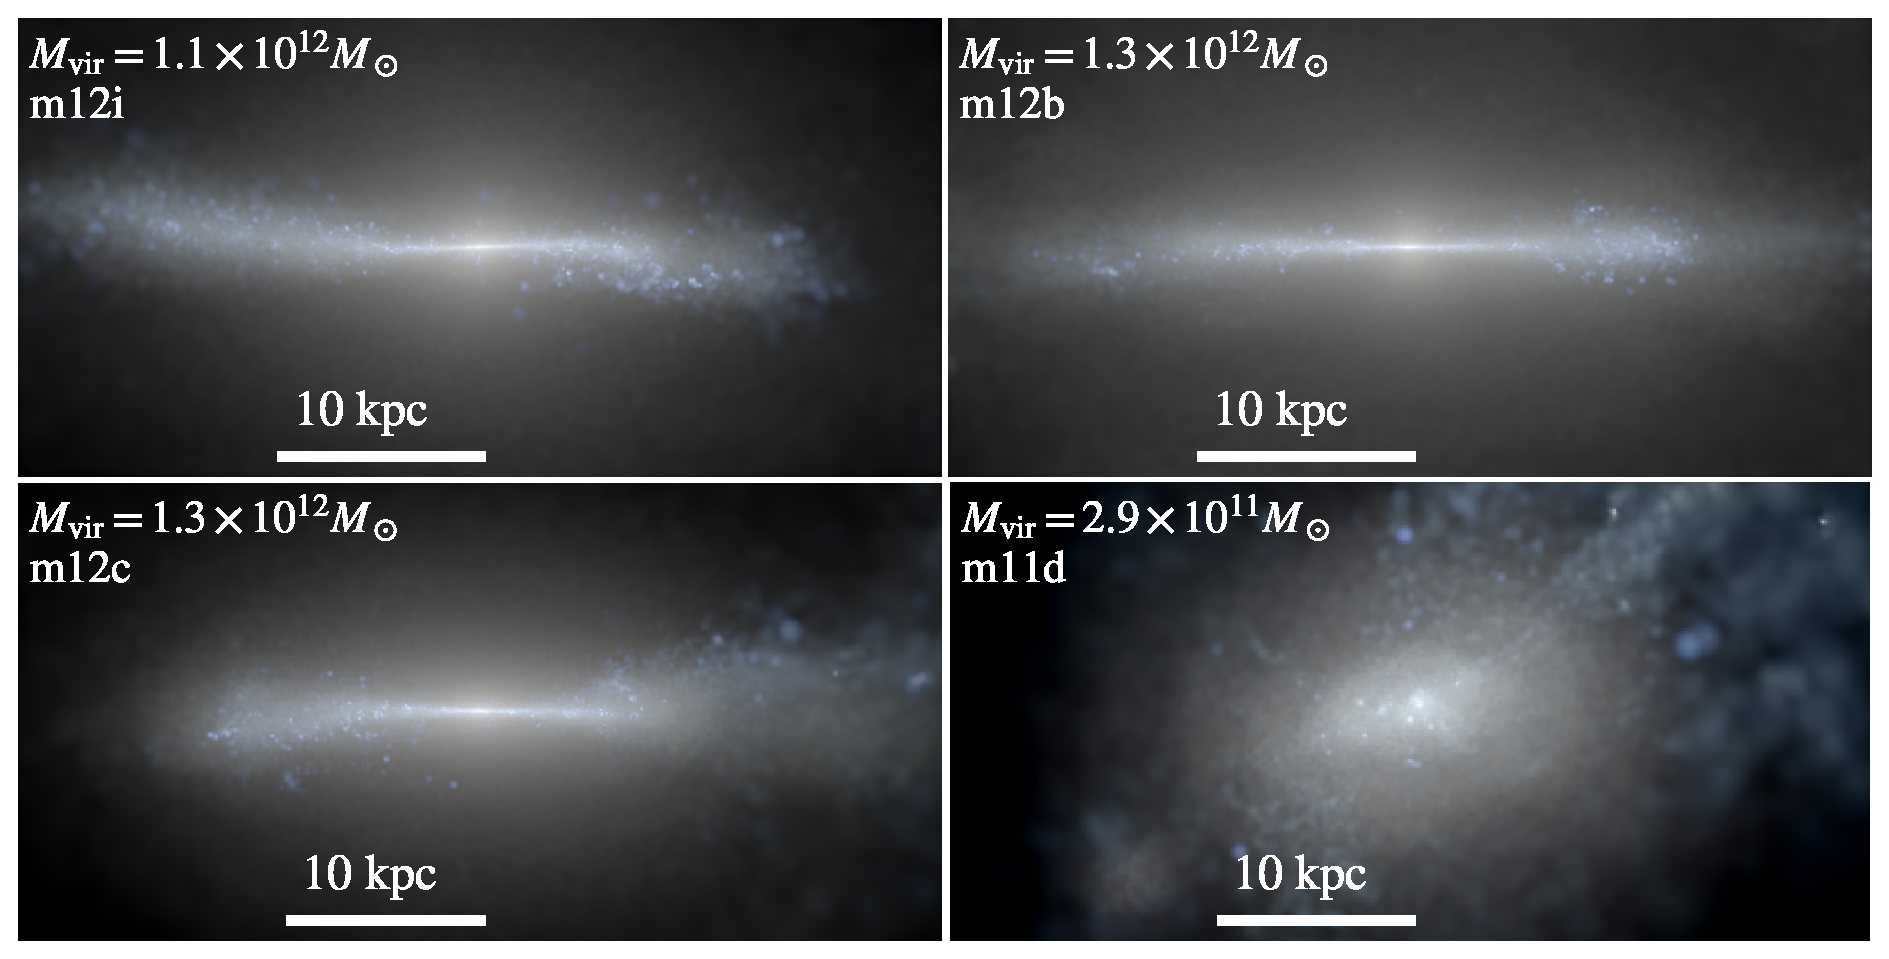
\includegraphics[width=\textwidth]{figures/stars.pdf}
    \caption{
    Mock Hubble images of four $z=0$ galaxies in the FIRE-2 simulations. Halo masses are noted in the panels, together with the fraction of young ($<1$ Gyr) stars which reside in a thin disc.  The Milky Way-mass galaxies have thin disc morphologies (top, bottom-left), while the lower mass galaxy has an irregular morphology (bottom-right).
    % \textbf{
    % Try changing dynamic range.
    % }
    }
    \label{f: stars}
\end{figure*}

% Basic disc formation idea, and its limitations
Our present picture for the formation of galactic discs can be largely traced to analytic ideas first explored by \citet{fall1980}, where a galaxy's angular momentum is intimately tied to the corresponding properties of its host dark matter halo.
Collapsing structures in an otherwise expanding universe will be spun up by the large-scale matter field \citep{Peebles69};
this can deliver enough angular momentum to allow (at least some) galaxies to have significant angular-momentum support~\citep[e.g.][]{MMW98}. 
While these ideas have provided foundational insights into the origin of disc galaxies in a $\Lambda$CDM universe, our understanding of disc  formation, and thin-disc galaxy formation in particular, remains incomplete. 
While dark matter haloes of all masses have similar angular momentum distributions \citep[e.g.][]{Barnes87}, disc fraction varies noticeably as a function of galaxy mass \citep[e.g.][]{Bernardi2010, Bluck2014, Moffett16}.
Moreover, dark matter spin alone is insufficient to explain the detailed properties of discs formed in cosmological simulations~\citep[e.g.][]{Sales2012, GK18}.  

% The puzzle of thin discs
Given what we know about the angular momentum distribution in galactic haloes, it is somewhat surprising that so many galaxies are dominated by {\em thin} discs, with  scale heights and vertical velocity dispersions that are small compared to their scale radii and circular speeds, $h/R \sim \sigma_z/V_c \sim 0.1$~\citep[][]{Kregel2002}.
We know, for example, that the angular momentum distribution of dark matter \citep{Bullock2001,Lian2018} and gas \citep{Stewart2013,DeFelippis2020} in galactic haloes is quite \textit{broad}.
This means that in order for a tightly-ordered thin disc to emerge, the gas must become coherently aligned along a single plane \textit{after} being part of the quasi-spherical extended galactic halo and \textit{before} forming stars.
This suggests that the process by which gas is deposited from the galactic halo into the galaxy, and how this process affects the angular momentum distribution, is an essential aspect of thin disc formation.

% Accretion
The process by which gas is deposited into a galaxy from the circumgalactic medium (CGM) has been the subject of considerable exploration~\citep[e.g.][]{Keres2005, Keres2009a, Dekel2006, Faucher-Giguere2011a, VanDeVoort2011a, Angles-Alcazar2017, Martin2019a} with broadly two paths to galaxy fueling identified: hot mode and cold mode.
In the cold-mode case, gas is deposited into the galaxy without ever virializing; this occurs typically in lower-mass haloes, where the gas cooling time is shorter than the infall time.
In hot-mode accretion, which dominates for massive haloes at late times ($M_{\rm vir} \gtrsim 10^{12} \Mdot$, $z \lesssim 1$; e.g. \citealt{Faucher-Giguere2011a, VandeVoort2011, VandeVoort2012a, Joung2012, Murante2012, Nelson2013, Fielding2017}), gas first shock-heats to the halo virial temperature, and then radiates its gravitational and thermal energy prior to accreting onto the galaxy.
Our own Milky Way (MW) is one such galaxy for which hot-mode accretion is expected to dominate.
As discussed above, we expect the mode of gas delivery, and the precise means by which gas mixes, cools, and accretes should have a substantial bearing on the ability to form thin, coherently rotating discs.  

% Cold mode
In cold mode accretion, cool ($T \sim 10^4$ K) gas travels from cosmological scales through the intergalactic medium (IGM) and into the galaxy in filaments~\cite[e.g.][]{Keres2005, Keres2009, Dekel2006, Faucher-Giguere2011a, Martin2019a}, often along with embedded satellite galaxies~\citep[e.g.][]{Faucher-Giguere2015, Faucher-Giguere2016, Hafen2019, Esmerian2021}.
This mode is expected to dominate the mass inflow rate at high redshifts \citep[$z\gtrsim2$; e.g.][]{Keres2009a, Dekel2009, Huscher2021}.
It is unclear, however, if the cool filaments remain intact down to the galaxy, or rather heat up and dissolve into the surrounding hot phase~\citep[e.g.][]{Nelson2016, Mandelker2016, Mandelker2018, Mandelker2020a}, in which case hot accretion onto the galaxy would also be important at high redshift.
While cool halo inflow of this kind typically contains more specific angular momentum (in total) than either hot gas or dark matter~\citep[e.g.][]{Stewart2017}, the tendency for such gas to reach the galactic region prior to mixing may hinder the ability to develop a thin, coherently aligned structure prior to star formation.
The fact that thin disc galaxies are common only among fairly massive systems ($L \sim 0.1 L_\star - L_\star$) at lower redshift~\citep[e.g.][]{Kranz2003, Kassin2006, Bizyaev2021, Kassin2012a, Simons2015, Simons2017}, suggests the idea that cold-mode delivery may not be conducive to thin disc formation.

% Hot mode
An alternative possibility is that hot-mode accretion, believed to dominate in more massive haloes at lower redshift, is more favorable to thin-disc formation.
This depends on the specific mechanics of this accretion mode, and on whether the hot gas manages to cool and accrete rather than being reheated by galactic feedback processes.
One possible subset of hot-mode accretion is instability-driven accretion, wherein gas precipitates out of the hot halo due to thermal instabilities, forming cool clouds that lose buoyancy and accrete onto the galaxy~\citep[e.g.][]{Maller2004, Mccourt2012, Voit2015, Armillotta2016, Gronke2020b,Fielding2020, Voit2021}.
Alternatively, radiative cooling in the hot CGM can cause the entire hot phase to flow inward.
In this latter scenario, the inward flow occurs at a rate where compression heating of the hot phase roughly balances radiative losses, so the hot gas roughly retains its temperature.
This type of hot accretion has been termed a `cooling flow' in the context of galaxy cluster studies~\citep[][see \citealt{McNamara2007} for a review]{Mathews1978, Cowie1980, Fabian1984, Balbus1988, Bertschinger1989}, and was recently revisited by \cite{Stern2019} in the context of galaxy-scale haloes.
\cite{Stern2020} then further explored the interplay between angular momentum and thermodynamics in these solutions, using steady-state calculations and idealised hydrodynamic simulations. 
In the present paper we demonstrate that such cooling flows with angular momentum (i.e. `rotating cooling flows')
are the primary mode of gas accretion onto discy Milky Way-mass galaxies at $z \sim 0$ in the FIRE-2 cosmological simulations \citep{Hopkins2018}, and may be a necessary condition for the formation of thin star-forming discs.

The analysis here follows \cite{Stern2021}, which showed that the formation of discs is closely connected to the formation of a virialized and stable hot CGM.
\cite{Yu2021} subsequently showed that the emergence of an inner virialized CGM correlates specifically with a transition from {\em thick}-disc to {\em thin}-disc formation.
The conditions necessary for stars to be born on circular orbits in a well-aligned plane appears to correlate with the conditions necessary for the onset of hot accretion modes such as cooling flows.
This finding partially motivates the exploration that follows.
Central to our analysis, and the analyses of \citeauthor{Stern2021} and \citeauthor{Yu2021}, are the FIRE simulations~(Feedback in Realistic Environments; \citealt{Hopkins2014, Hopkins2018})\footnote{\url{https://fire.northwestern.edu/}} a set of ``zoom-in'' simulations that resolve stellar feedback on the scale of giant molecular clouds in the interstellar medium (ISM)~\citep{Guszejnov2020b, Benincasa2020}, producing winds that naturally expand into the CGM and interact with accreting gas~\citep{Muratov2015, Muratov2017, Angles-Alcazar2017, Hafen2019, Hafen2020, Pandya2021}.
The resultant galaxies are broadly consistent with the stellar mass-halo mass relation~\citep{Hopkins2017}, satellite galaxy populations~\citep{Wetzel2016, Garrison-Kimmel2019a, Samuel2020}, and can have thin-discs consistent with Milky Way-like galaxies~\citep{Ma2017a, Garrison-Kimmel2018, El-Badry2018, Sanderson2020, Yu2021}.

Here we use the FIRE-2 simulations to study gas accretion onto $z\sim0$ galaxies and its relation to thin disc morphology.
Our approach uses the particle-tracking methodology developed in \citet{Hafen2019, Hafen2020} to explore the mechanics of rotating cooling flows near the disc-halo interface where angular momentum support is substantial.
This goes beyond 1D steady-state solutions developed in classic ICM studies~\citep[e.g.][]{Cowie1980}, and extends the idealised 3D simulations in \cite{Stern2019} to a more realistic cosmological setting. 
Our work is complementary to \citet{Trapp2021}, who characterized in-depth the phenomenological properties of accretion onto MW-like FIRE galaxies, and the particle tracking analysis of \cite{Angles-Alcazar2017}, who provided an overview of the connection between the cosmic baryon cycle and galaxy mass assembly. 

% This paper
This paper is structured as follows. 
In \S\ref{s: methods} we describe our sample of FIRE simulations and the sample of accreting particles selected from the simulations.
In \S\ref{s: results} we analyse the characteristics and mechanics of gas accretion onto $z\sim0$ galaxies in FIRE, and their relation to thin disc morphology in the central galaxy.
We discuss our results in \S\ref{s: discussion} and conclude in \S\ref{s: conclusions}.

\section{Methods}
\label{s: methods}

\subsection{Simulations}
\label{s: methods -- simulations}

\begin{table*}
\caption{Simulation parameters.}
\begin{tabular}{cccccccc}
\hline
Name  &  $f_{\rm thin\,disc,\,recent}$  & $M_{\rm vir}$  &  $M_\star$  &  $R_{\textrm{vir}}$  &  $\Delta f_{\rm aligned}$  &  Metal diffusion?  &  Reference  \\
  &   & $M_\odot$  & $M_\odot$  &  kpc  &  &  &  \\
 \hline
m12i  &  0.83  &  $1.1\times10^{12}$  &  $7.3\times10^{10}$  &  268  &  0.34  &  \checkmark  &  \cite{Wetzel2016}    \\
m12b  &  0.8  &  $1.3\times10^{12}$  &  $1.0\times10^{11}$  &  286  &  0.35  &  \checkmark  &  \cite{Garrison-Kimmel2019a}    \\
m12i\_core  &  0.79  &  $1.1\times10^{12}$  &  $8.0\times10^{10}$  &  274  &  0.34  &    &  \cite{Hopkins2018}    \\
m12c  &  0.72  &  $1.3\times10^{12}$  &  $6.8\times10^{10}$  &  283  &  0.25  &  \checkmark  &  \cite{Garrison-Kimmel2019a}    \\
m12f  &  0.72  &  $1.5\times10^{12}$  &  $9.7\times10^{10}$  &  302  &  0.24  &  \checkmark  &  \cite{Garrison-Kimmel2017}    \\
m12m  &  $^*$0.37  &  $1.5\times10^{12}$  &  $1.4\times10^{11}$  &  298  &  0.26  &    &  \cite{Hopkins2018}    \\
m12w  &  0.33  &  $9.5\times10^{11}$  &  $6.5\times10^{10}$  &  253  &  0.15  &  \checkmark  &  \cite{Samuel2020}    \\
m11h  &  0.24  &  $1.8\times10^{11}$  &  $3.9\times10^{9}$  &  146  &  0.047  &  \checkmark  &  \cite{El-Badry2018a}    \\
m11b  &  0.2  &  $4.4\times10^{10}$  &  $1.2\times10^{8}$  &  92.4  &  0.12  &    &  \cite{Chan2018}    \\
m12r  &  0.16  &  $1.0\times10^{12}$  &  $2.4\times10^{10}$  &  257  &  0.11  &  \checkmark  &  \cite{Samuel2020}    \\
m12z  &  0.073  &  $8.0\times10^{11}$  &  $2.5\times10^{10}$  &  242  &  0.052  &  \checkmark  &  \cite{Garrison-Kimmel2019a}    \\
m11e  &  0.05  &  $1.5\times10^{11}$  &  $1.6\times10^{9}$  &  136  &  0.044  &  \checkmark  &  \cite{El-Badry2018a}    \\
m11i  &  0.023  &  $7.0\times10^{10}$  &  $1.0\times10^{9}$  &  106  &  0.013  &  \checkmark  &  \cite{El-Badry2018a}    \\
m11a  &  0.018  &  $4.1\times10^{10}$  &  $1.3\times10^{8}$  &  90.3  &  -0.022  &    &  \cite{Chan2018}    \\
m11c  &  0.015  &  $1.4\times10^{11}$  &  $9.5\times10^{8}$  &  137  &  0.0068  &    &  \cite{Hopkins2018}    \\
m11d  &  0.0097  &  $2.9\times10^{11}$  &  $4.9\times10^{9}$  &  169  &  0.0026  &  \checkmark  &  \cite{El-Badry2018a}    \\
m11q  &  0.0058  &  $1.5\times10^{11}$  &  $7.4\times10^{8}$  &  138  &  0.0045  &  \checkmark  &  \cite{Hopkins2018}    \\ %\hline
% m12i\_cr  &  0.81  & $1.1\times10^{12}$  &  $6.5\times10^{10}$  &  270  &  0.27  &  CR+  &  ?    \\
\end{tabular}
\\
\begin{flushleft}
Properties at $z=0$ of the sample of FIRE galaxies analysed in this work.
The value of $f_{\rm thin\,disc,\,recent}$ is the fraction of stars formed in the last Gyr prior to $z=0$ that are in a thin disc configuration ($j/j_c(E) > 0.8$; e.g. \citealt{Yu2021}).
Note that the \texttt{m12m} galaxy (marked by $^*$) has a sizable bar, which forms secularly at late times and drives the thin-disc fraction lower by our adopted definition~\citep{Debattista2019}..
The value of $\Delta f_{\rm aligned}$ is a measure of the relation between cooling and circularization in accreted gas (\S\ref{s: characteristics -- aligns}).
The ``Metal diffusion?'' column marks whether or not the simulation includes a subgrid prescription for metal diffusion.
% The ``hydro+'' simulations include fiducial FIRE-2 physics, while the ``no MD'' simulations exclude a prescription for subgrid metal diffusion.
\end{flushleft}
\label{table: simulations_used}
\end{table*}

% FIRE simulations
We analyse the hydrodynamical cosmological zoom-in simulations produced as part of the FIRE project~\citep{Hopkins2014}.
The simulation sample, listed in Table~\ref{table: simulations_used}, were run with the FIRE-2 version~\citep{Hopkins2018} of the gravity and hydrodynamics code \textsc{GIZMO}\footnote{\url{http://www.tapir.caltech.edu/\~phopkins/Site/GIZMO.html}}~\citep{Hopkins2015}.
The simulations were produced using the meshless finite-mass (``MFM'') mode of \textsc{GIZMO}, a Lagrangian method with no inter-element mass flux.
This enables use to track the history of each resolution element.
The full details of simulations produced with the FIRE-2 code are available in~\cite{Hopkins2018}.
The FIRE simulations include detailed prescriptions for star formation and stellar feedback.
Each star particle contributes to the simulation momentum from radiation pressure; energy, momentum, mass, and metals from Type Ia and II supernovae and stellar winds; and photo-ionization and photo-electric heating.
Star formation is limited to self-gravitating, self-shielding (molecular) gas with a density of at least $n_{\rm SF} = 1000$ cm$^{-3}$.
In addition to stellar radiation, the simulations include a uniform meta-galactic radiation background that ionizes gas in the intergalactic medium~\citep{Faucher-Giguere2009}.
In the simulations and throughout our analysis we use a standard flat $\Lambda$CDM cosmology with $\Omega_{\rm m }\approx 0.32$, $\Omega_{\Lambda}=1-\Omega_{\rm m}$, $\Omega_{\rm b} \approx 0.049$, and $H_{0} \approx 67$ km s$^{-1}$ Mpc$^{-1}$~\citep[e.g.,][]{PlanckCollaboration2018}.

% Figure 1
Figure~\ref{f: stars} shows edge-on mock Hubble images (though neglecting dust attenuation to more clearly illustrate the stellar distribution) for the $z=0$ snapshots of four of our simulated galaxies.
The top and bottom-left panels show three MW-mass galaxies (\texttt{m12i}, \texttt{m12b}, and \texttt{m12c}) while the bottom-right panel shows a $M_\star \sim 5 \times 10^9 M_\odot$ dwarf galaxy, \texttt{m11d}.
As noted in previous studies~\citep{Garrison-Kimmel2018, El-Badry2018} MW-mass galaxies in FIRE typically have thin disc morphologies, while lower mass galaxies show a thick disc / irregular morphology.
We quantify this trend using $f_{\rm thin\,disc,\,recent}$, defined as the fraction of stars with age $<1$ Gyr (at $z=0$) that have $j_z/j_c(E) > 0.8$~\citep[e.g.][]{Yu2021}.
Here $j_z$ is the specific angular momentum in the $z$ direction and $j_c(E)$ is the angular momentum the star would have if it had the same energy but was in a circular orbit.
The $z$ axis is defined as the direction of the total angular momentum vector of stars inside the galaxy.
This definition of the thin disc is the same definition used in~\cite{Yu2021}.
Values of $f_{\rm thin\,disc,\,recent}>0.8$ correspond to height to size ratios $h/R \sim 0.1$ and rotation to dispersion ratios $V_{\rm rot}/\sigma_z \sim10$, and correlate strongly with the observed thin disc fraction in the $r$ band (appendix \ref{s: appendix-sloan thin disc fraction}).
The values of $f_{\rm thin\,disc,\,recent}$ are noted in Fig.~\ref{f: stars} and listed in Table~\ref{table: simulations_used}.

\subsection{Analysis}
\label{s: methods -- analysis}

% How we select the particles
For each galaxy we use the particle tracking method described in \cite{Hafen2019, Hafen2020}, which in turn built on insight from previous particle-tracking applied to the FIRE simulations~\citep{Angles-Alcazar2017}.
We select an unbiased sample of resolution elements (particles) that have accreted onto the central galaxy during the last Gyr prior to $z=0$.
To select such particles, we require that they are
(1) within the galaxy radius $r_{\rm gal}$ at $z=0$, either in stars or in gas with density  $n_{\rm H} > 0.13$ cm$^{-3}$, and
(2) within the CGM (gas at $0.1 - 1 \Rvir$) in the snapshot corresponding to 1 Gyr prior to $z=0$.
Throughout the paper we use $r$ for the 3D distance. 
We define $r_{\rm gal} = 4 r_{\star,0.5}$ following \cite{Hafen2019, Hafen2020}, where $r_{\star, 0.5}$ is the stellar half-mass radius.
For each selected particle we retrieve the full history of the particle (including temperature, density, and metallicity). 
We discard a small fraction ($<2\%$) of the particles whose mass increases by a factor two as a natural consequence of mass deposition by stellar feedback.
These particles pose a problem for our tracking method because the history of the additional mass is not recorded, and because they are split into multiple particles after gaining sufficient mass.

% Definition of t1e5 and calculating it
A key time for our analysis is the last time a particle cools prior to entering the galaxy.
For a given particle, we define this time as:
\begin{equation}
    \tcools \equiv t \bigg( {\rm last\,snapshot\,outside\,galaxy\,with\,}T>10^5\,{\rm K} \bigg) ~,
\label{e: tcools}
\end{equation}
i.e., the last snapshot the particle was hot prior to entering the galaxy (according to the galaxy definition above).
For gas that cools as it accretes, $\tcools$ occurs as the gas passes through the galaxy-halo interface.
Below we analyse the statistical properties of all accreting particles as a function of time relative to their cooling time ($t-\tcools$).

\section{Results}
\label{s: results}

% INTUITIVE OVERVIEW
\begin{figure*}
    \centering
    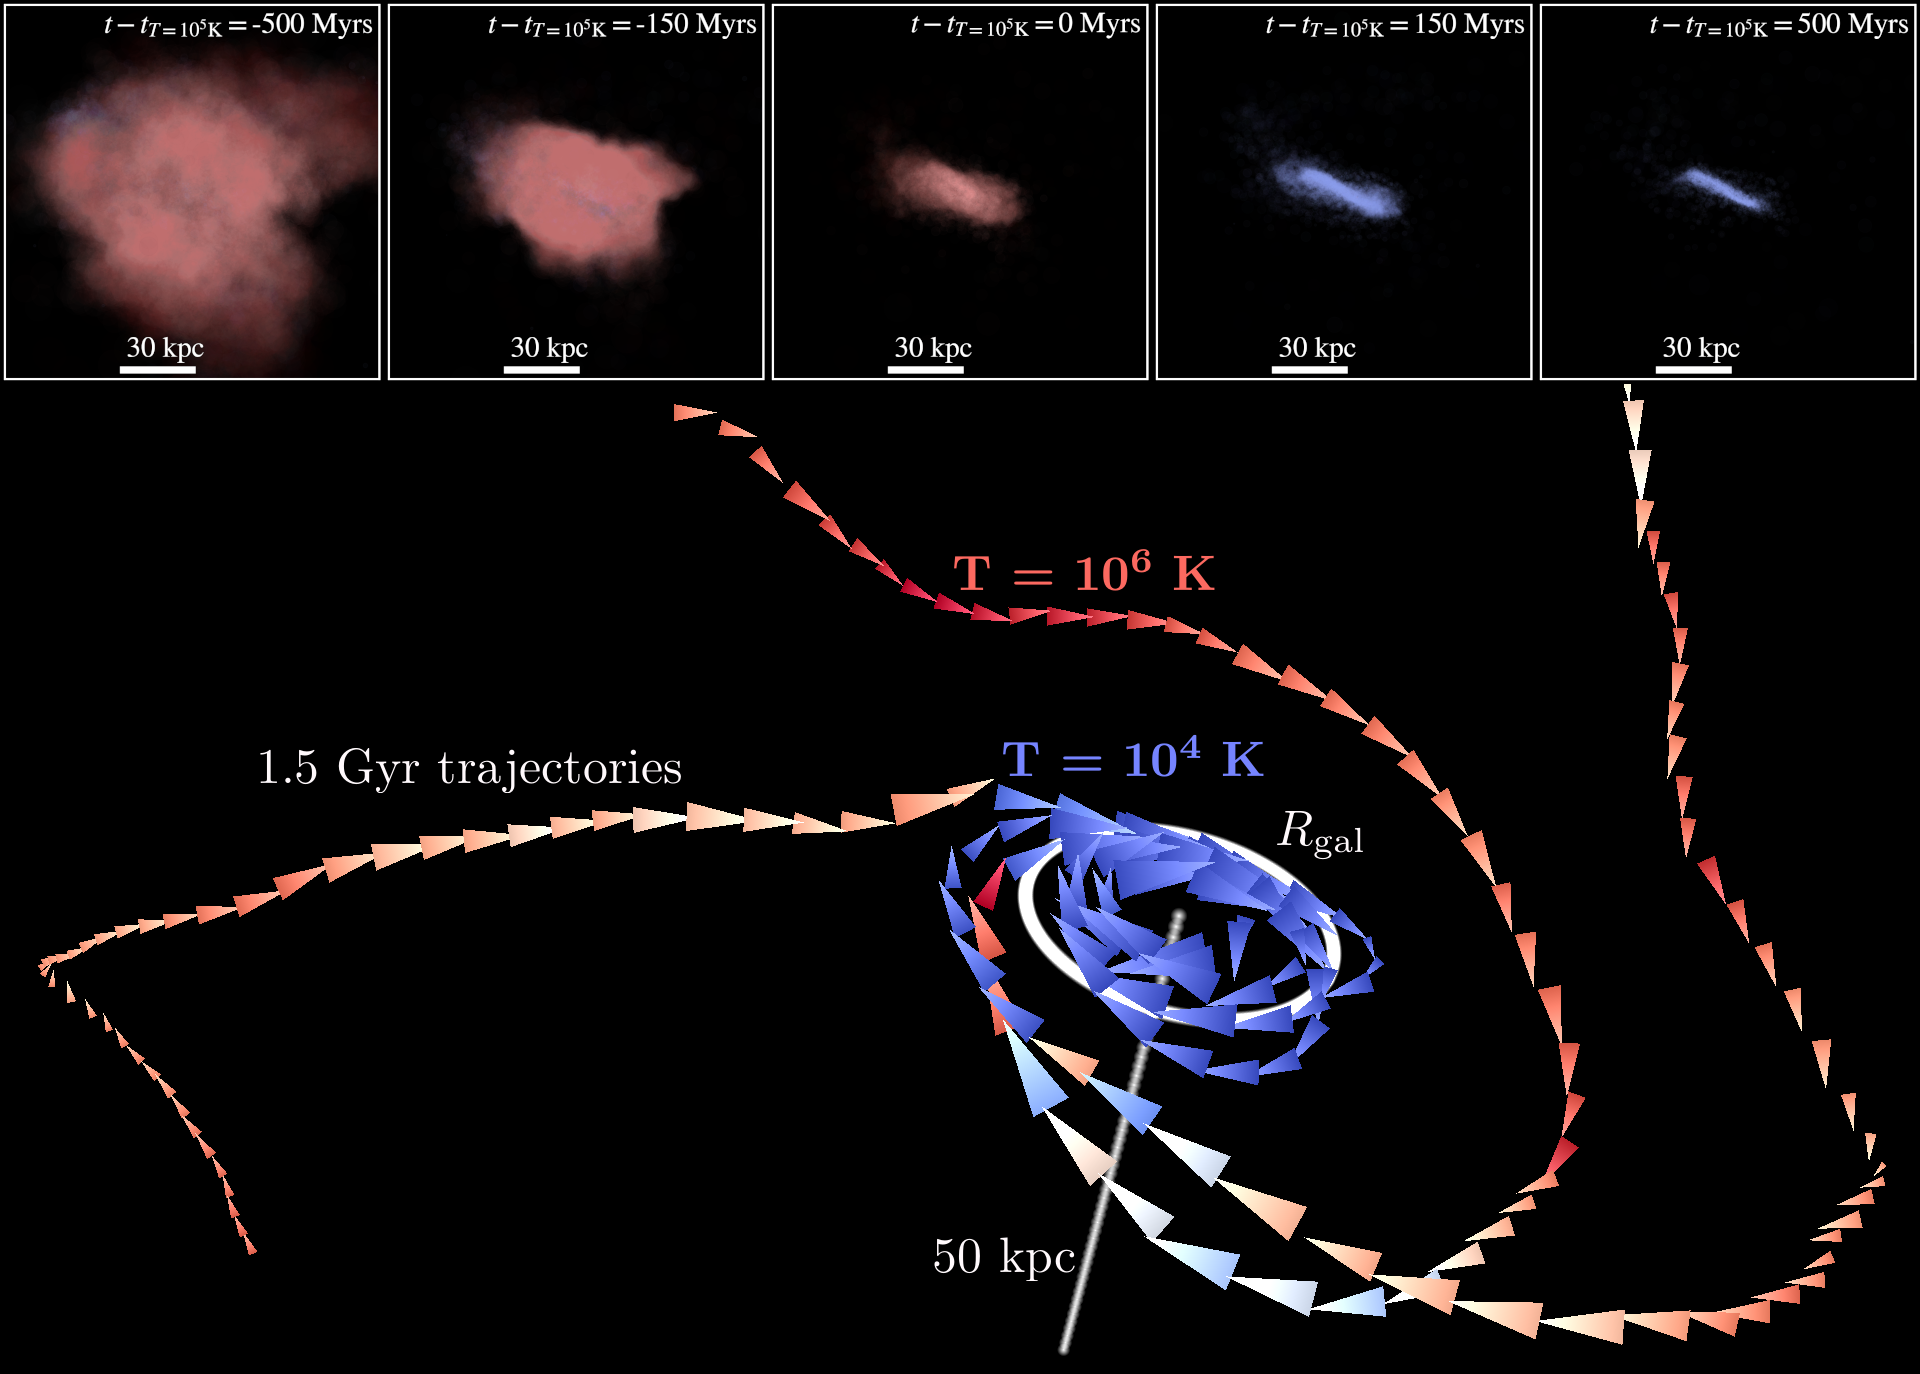
\includegraphics[width=\textwidth]{figures/illustrative_tracks/illustrative_tracks.png}
    \caption{
Gas accretion onto a Milky Way-mass disc galaxy in FIRE, \texttt{m12i}, near $z\approx0$.
\textbf{Top and right panels:}
Temperature and spatial evolution of accreting gas with respect to $\tcools$, defined as the last time at which the gas cools below $10^5$ K prior to accreting onto the galaxy.
Red, white, and blue indicates $T=10^6$ K, $10^5$ K, and $10^4$ K respectively. 
\textbf{Bottom-left panel:}
Three representative trajectories for accreting gas elements.
The panels show that accretion is hot ($\approx 10^6$ K) and contracts quasi-spherically at early times relative to the cooling time.
At the time of cooling the geometry of accreting gas transitions from a quasi-spherical distribution at $t-\tcools < -150$ Myr to a cool disc at $t-\tcools > 150$ Myr.
    }
    \label{f: overview}
\end{figure*}

% Summary picture description
To characterize gas accretion we analyse the central galaxy and its CGM from $z=0$ to one Gyr prior.
Figure~\ref{f: overview} shows a visual overview of how gas accretes onto \texttt{m12i} -- a MW-mass galaxy that forms a substantial thin disc ($f_{\rm thin\,disc,\,recent} = 0.83$). 
The top and right panels plot the temperature and spatial evolution of accreting gas versus time prior to cooling ($t-\tcools$), while the bottom-left panel plots three representative trajectories for accreting gas elements.
The trajectories were visualized using the Firefly visualization software~\citep{Geller2018}.
\footnote{See the Firefly homepage at \url{galaxies.northwestern. edu/firefly}.
A 3D version of the trajectories is available online at \url{zhafen.github.io/rotating-cooling-flows}.}
The trajectory color scales with temperature, with red, white, and blue indicating $T=10^6$ K, $10^5$ K, and $10^4$ K, respectively.
The figure shows that at early times relative to cooling ($t-\tcools \sim -1000$ Myr) the accretion is hot ($\approx10^6$ K) and contracts quasi-spherically.
Then, around the time of cooling the geometry of accreting gas transitions from quasi-spherical at $t - \tcools=-150$ Myr to a cool disc aligned with the galaxy (not shown) at $t - \tcools=+ 150$ Myr.
A quantitative analysis of this transition follows in sections \ref{s: characteristics -- inflowing gas phase}--\ref{s: mechanics -- energy balance}.

\subsection{Gas inflow onto thin-disc MW analogs is hot through the CGM}
\label{s: characteristics -- inflowing gas phase}

Figure~\ref{f: before and after A} plots various characteristics of accreting gas on the \texttt{m12i} thin disc galaxy, as a function of time relative to the accretion's last cooling time ($t - \tcools$).
In each panel, solid lines and shaded regions mark the medians and 16th to 84th percentile ranges of all particles accreted within $0.5-1$ Gyr prior to $z=0$.
The lower limit on the time range applied in this figure is to ensure that particles are present for most of the time displayed after $\tcools$, although removing the limit does not change the qualitative results.
In the temperature panel (A) we exclude from the distribution particles that have converted into stars. 

Panel (A) demonstrates that during the 500 Myr prior to cooling for a final time, the inflow is predominantly hot ($\gtrsim 10^5$ K), with a median temperature of $4-8\times10^5$ K, similar to the halo virial temperature of $\Tvir(z=0)=6.5\times10^5$ K.
This is not true by construction --- gas may have been heated only shortly before cooling.
During this time prior to cooling the accreting gas is inflowing toward the galaxy (panel B), from a median $r=55$ kpc at $t-\tcools=-500$ Myr, to a median $r\approx18\,{\rm kpc}\approx1.4 r_{\rm gal}$ at $t=\tcools$, after which time the inflow stalls.
The characteristic inflow velocity of $v_r \approx-70$ km s$^{-1}$ (Panel D) is substantially lower than the circular velocity of $170-200$ km s$^{-1}$.
This radial velocity is also smaller than the median sound speed of $100-130$ km s$^{-1}$, indicating a subsonic radial flow. 


A similar hot inflow is seen in other thin disc galaxies in our sample (appendix~\ref{s: appendix-other m12s}).
Thus, accretion from the CGM onto $z=0$ thin discs in FIRE is dominated by the inflow of hot, virial temperature gas.
We show below that this accretion flow corresponds to a `cooling flow', similar to the classical solution envisioned for the ICM (e.g., \citealt{Mathews1978}).
Also, we emphasize that this hot accretion mode, in which the entire hot phase inflows, is qualitatively different from `precipitation' in which gas clumps cool at halo scales, lose buoyancy and subsequently accrete (e.g.~\citealt{Maller2004,Voit2017}). The dominance of hot accretion over precipitation in MW-like galaxies simulated in FIRE has previously been noted by \cite{Esmerian2021}. 

% CHARACTERISTICS OF QUIET ACCRETION
\begin{figure*}
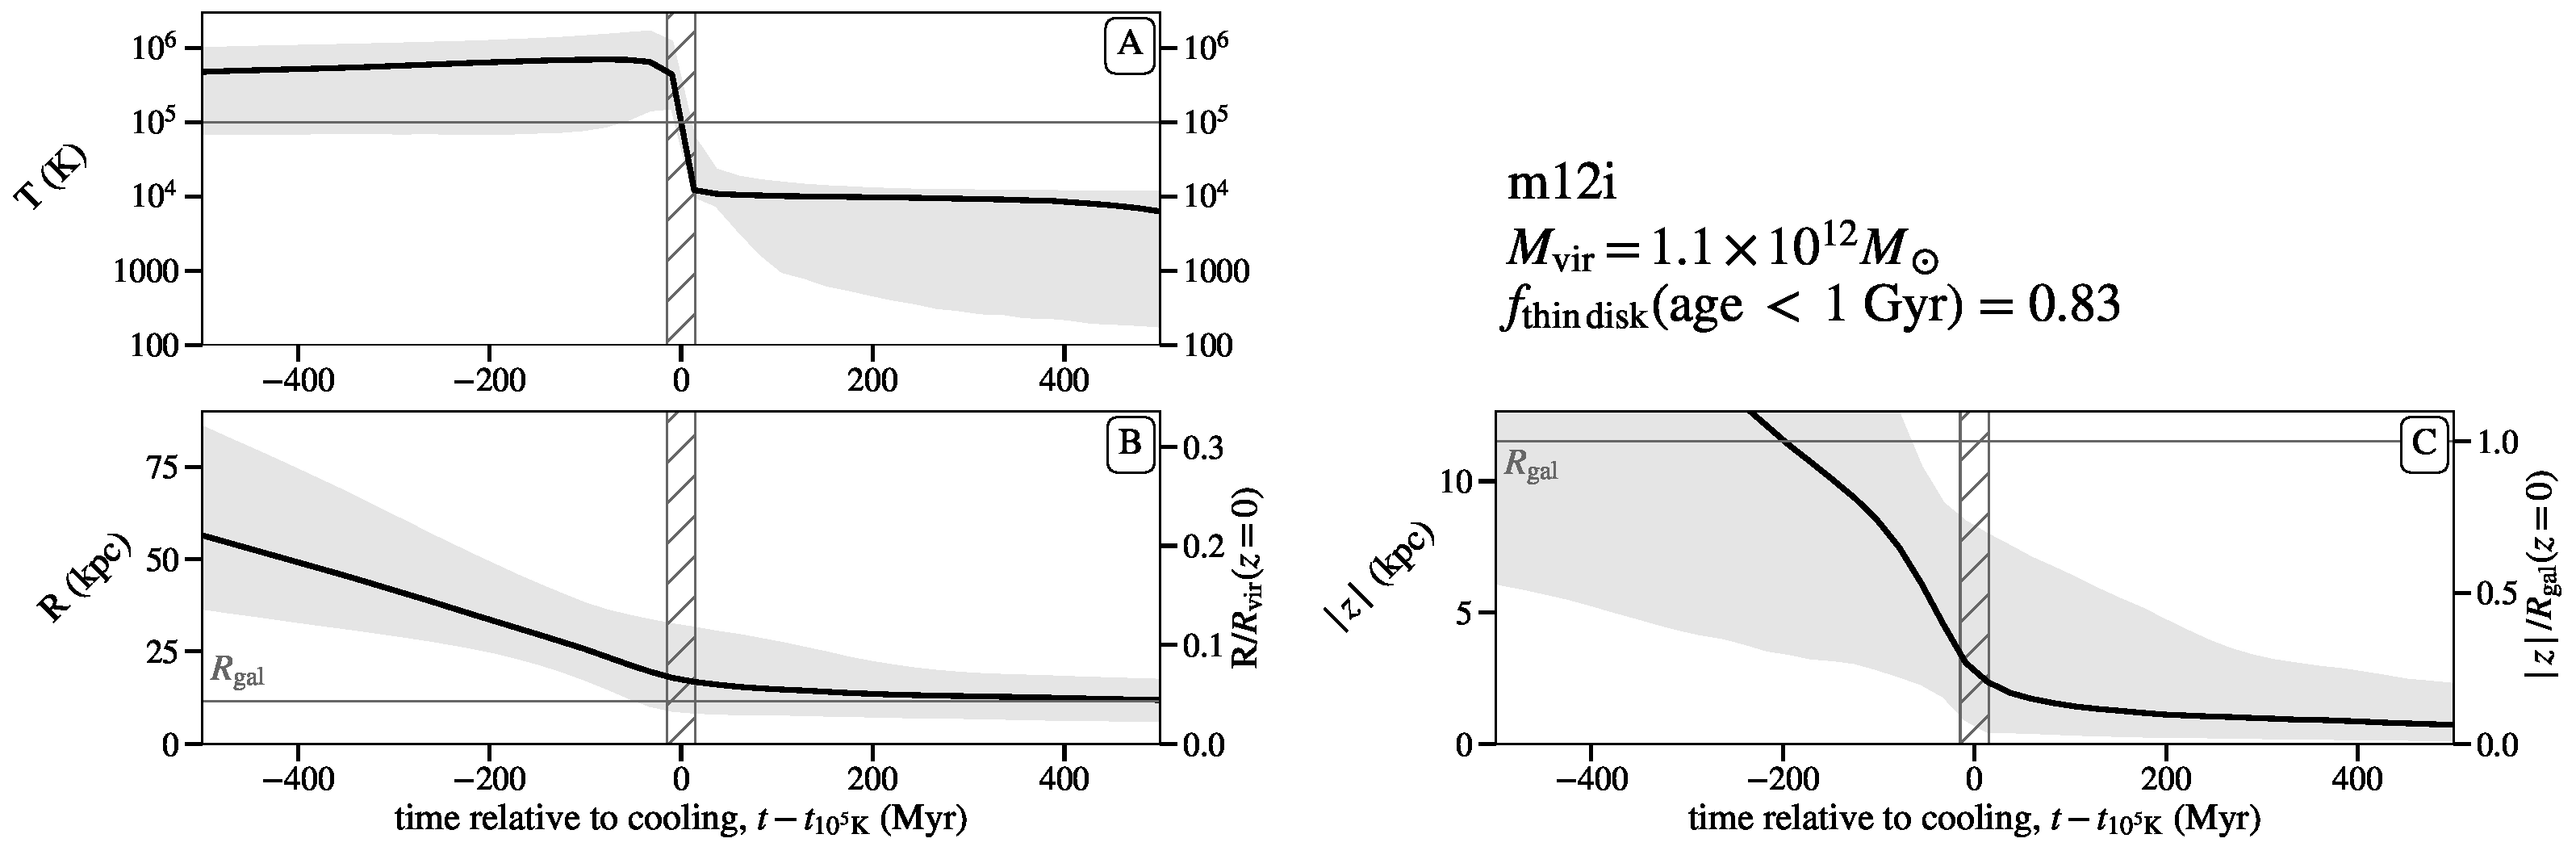
\includegraphics[width=\textwidth]{figures/before_and_after/before_and_after_characteristics_m12i_md.pdf}
\caption{
Properties of gas accretion onto a $z\sim0$ thin disc galaxy in FIRE, versus time relative to the final cooling time ($t - \tcools$).
In each panel solid lines and shaded regions mark the medians and 16th to 84th percentile ranges of all particles accreted within 1 Gyr prior to $z=0$. 
\textbf{A:}
Temperature.
During the 500 Myr prior to cooling, the inflow is predominantly hot ($\gtrsim 10^5$ K), with a median temperature approaching $\Tvir\approx10^6$ K.
At $t = \tcools$ the gas cools (by definition), and achieves cool ISM temperatures or forms stars at later times. 
\textbf{B:}
Distance from halo center (green) and absolute height from the disc plane (blue).
Cooling occurs at $r=10-30$ kpc, corresponding to $0.7-2.5\,r_{\rm gal}$.
Prior to cooling the gas forms an inflow while after cooling the inflow stalls.
Absolute height from the disc plane.
Most of the gas collapses into a disc upon cooling, with a median $\vert z \vert \approx 2$ kpc at $t=\tcools$.
\textbf{C:}
Velocity components of accretion (colored lines and band), relative to circular velocity at the median radius (dash-dotted line).
The gas reaches full rotational support upon cooling.
\textbf{D:}
Fraction of gas converted into stars.
Star formation starts after cooling, at a rate of $\sim10\%$ per $100$ Myr. 
}
\label{f: before and after A}
\end{figure*}


\subsection{Accretion cools and stalls at the galaxy-halo interface}
\label{s: characteristics -- cools}

Panel (A) in Fig.~\ref{f: before and after A} demonstrates that at $t = \tcools$ the temperature drops quickly from $\sim10^6$ K to $\sim10^4$ K.
Panel (B) shows that this cooling occurs just outside the galaxy, at $r(\tcools) \approx 10-30$ kpc, equivalent to $\approx0.7 - 2.5 r_{\rm gal}$\footnote{Note that gas can have $r(\tcools) < r_{\rm gal}$ if it is under-dense relative to the galaxy when it crosses $r_{\rm gal}$ ($n_{\rm H} < 0.13$ cm$^{-3}$), see section \ref{s: methods -- analysis}.}.
Less than $10\%$ of particles cool beyond $\sim 40$ kpc.
After cooling to $T \sim 10^4$ K, the temperature further drops to cool ISM temperatures of $100-10^4$ K and stars begin to form at a rate of $\approx10\%$ per $100$ Myr (panel E), roughly equal to the average rate in the galaxy ISM. 

Panel (D) in Fig.~\ref{f: before and after A} demonstrates that cooling at the galaxy scale is further associated with a change in accretion kinematics.
The z-axis is oriented along the total angular momentum of stars in the galaxy at $z=0$.
The radial inflow velocity $\vert v_r \vert $ starts decelerating $\approx40$ Myr prior to cooling, and almost completely stalls ($\lesssim10$ km s$^{-1}$) after cooling.
This stalling behavior was previously identified by \citet{Trapp2021}.
The stalling is associated with $v_\phi$ reaching $v_c$, indicating a transition from pressure-support in the hot CGM to rotational support in the cool ISM.
Note that deceleration prior to accretion is possible due to the subsonic nature of the radial hot flow --- the gas pressure can increase closer to the galaxy, slowing the inward movement.
Similar results are seen for accretion onto other thin-disc galaxies in our sample (appendix \ref{s: appendix-other m12s}). 
Specifically, the majority of accretion onto $z\sim0$ thin disc galaxies in FIRE is a hot inflow which cools and stalls just outside the galaxy.
This is {\em not} the case for galaxies that lack thin discs in our sample (appendix \ref{s: appendix-low mass}).
Galaxies that are dominated by thick/irregular morphology demonstrate no such stalling behavior.


\subsection{Cooling of accreted gas is concurrent with circularization}
\label{s: characteristics -- aligns}

% ORIENTS AS IT COOLS
\begin{figure*}
    \centering
    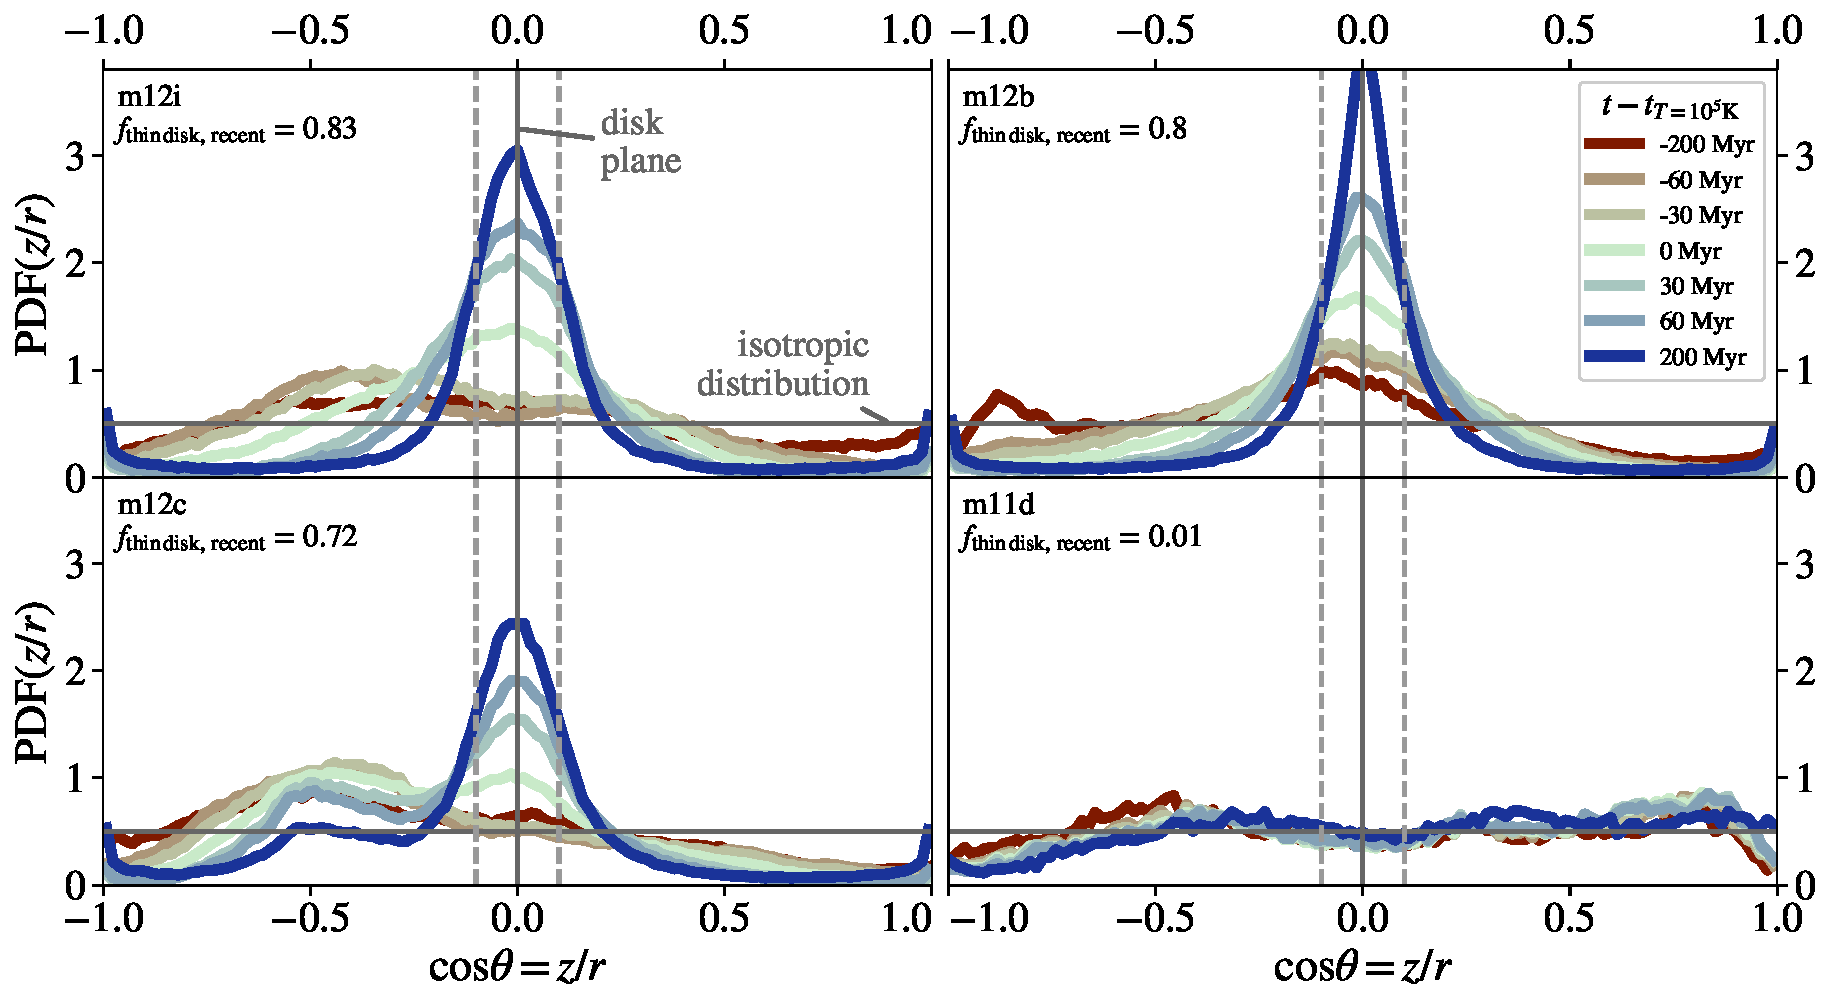
\includegraphics[width=\textwidth]{figures/theta_vs_t.pdf}
    \caption{
    Angular distribution of accreting gas, as a function of time relative to the last cooling time.
    In thin disc galaxies (top and bottom-left panels) the angular distribution of accreting gas evolves significantly at the time of cooling, from a quasi-spherical distribution prior to cooling to a disc-like configuration after cooling. 
    In contrast, in the irregular galaxy (bottom-right) accreting gas is roughly spherical both prior to and after cooling.
    }
    \label{f: theta vs t}
\end{figure*}

% Figure description/introduction
Panel (C) in Fig.~\ref{f: before and after A} plots the distance $z$ above the disc plane as a function of time.
We see that as the gas collapses, it becomes increasingly flattened in the disc plane.
The horizontal line shows $r_{\rm gal}$ for reference.
At the time of cooling, the gas has median height of $\approx 2$ kpc, indicating a disc geometry with height to radius ratio of $\vert z\vert/r_{\rm gal}\approx0.2$, consistent with the transition to rotation support indicated by panel (D).
Panel (E) in Fig.~\ref{f: before and after A} emphasizes that all of the star formation occurs after rotation support is achieved and the disc geometry is in place.

This correspondence between a transition to disc geometry and cooling is further explored in Figure~\ref{f: theta vs t}, which plots the geometry of accreting gas at different times relative to $\tcools$, for the four galaxies shown in Fig.~\ref{f: stars}. 
Times prior to cooling are colored in red, while times after cooling are plotted in blue.
All particles with $t-\tcools$ within $\pm$30 Myr of the value noted in the legend are included in the distribution. 
The curves show the PDF of $\cos \theta = z/r$, i.e.\ $\theta$ is the angle between the gas element position and the total angular momentum vector of stars in the galaxy at $z=0$.
A spherical distribution of accreted gas would have a flat PDF with a value of 0.5, while 
the PDF of an infinitely thin disc would be a $\delta$-function centered at $z/r = 0$.
The figure shows that gas accreting onto the three thin-disc galaxies transitions from being distributed quasi-spherically at $t = \tcools-200$ Myr to being distributed in the galaxy plane at $t = \tcools+200$ Myr.
This indicates that cooling and flattening of the accreted gas occurs simultaneously in these galaxies, consistent with the conclusion from Figs.~\ref{f: overview} and \ref{f: before and after A}.
In contrast, in the irregular galaxy shown in the bottom-right, there is no association between cooling and flattening.
Rather, the geometry of accreting gas is quasi-spherical both before and after cooling.

% PREVALENCE OF QUIET ACCRETION
\begin{figure*}
    \centering
    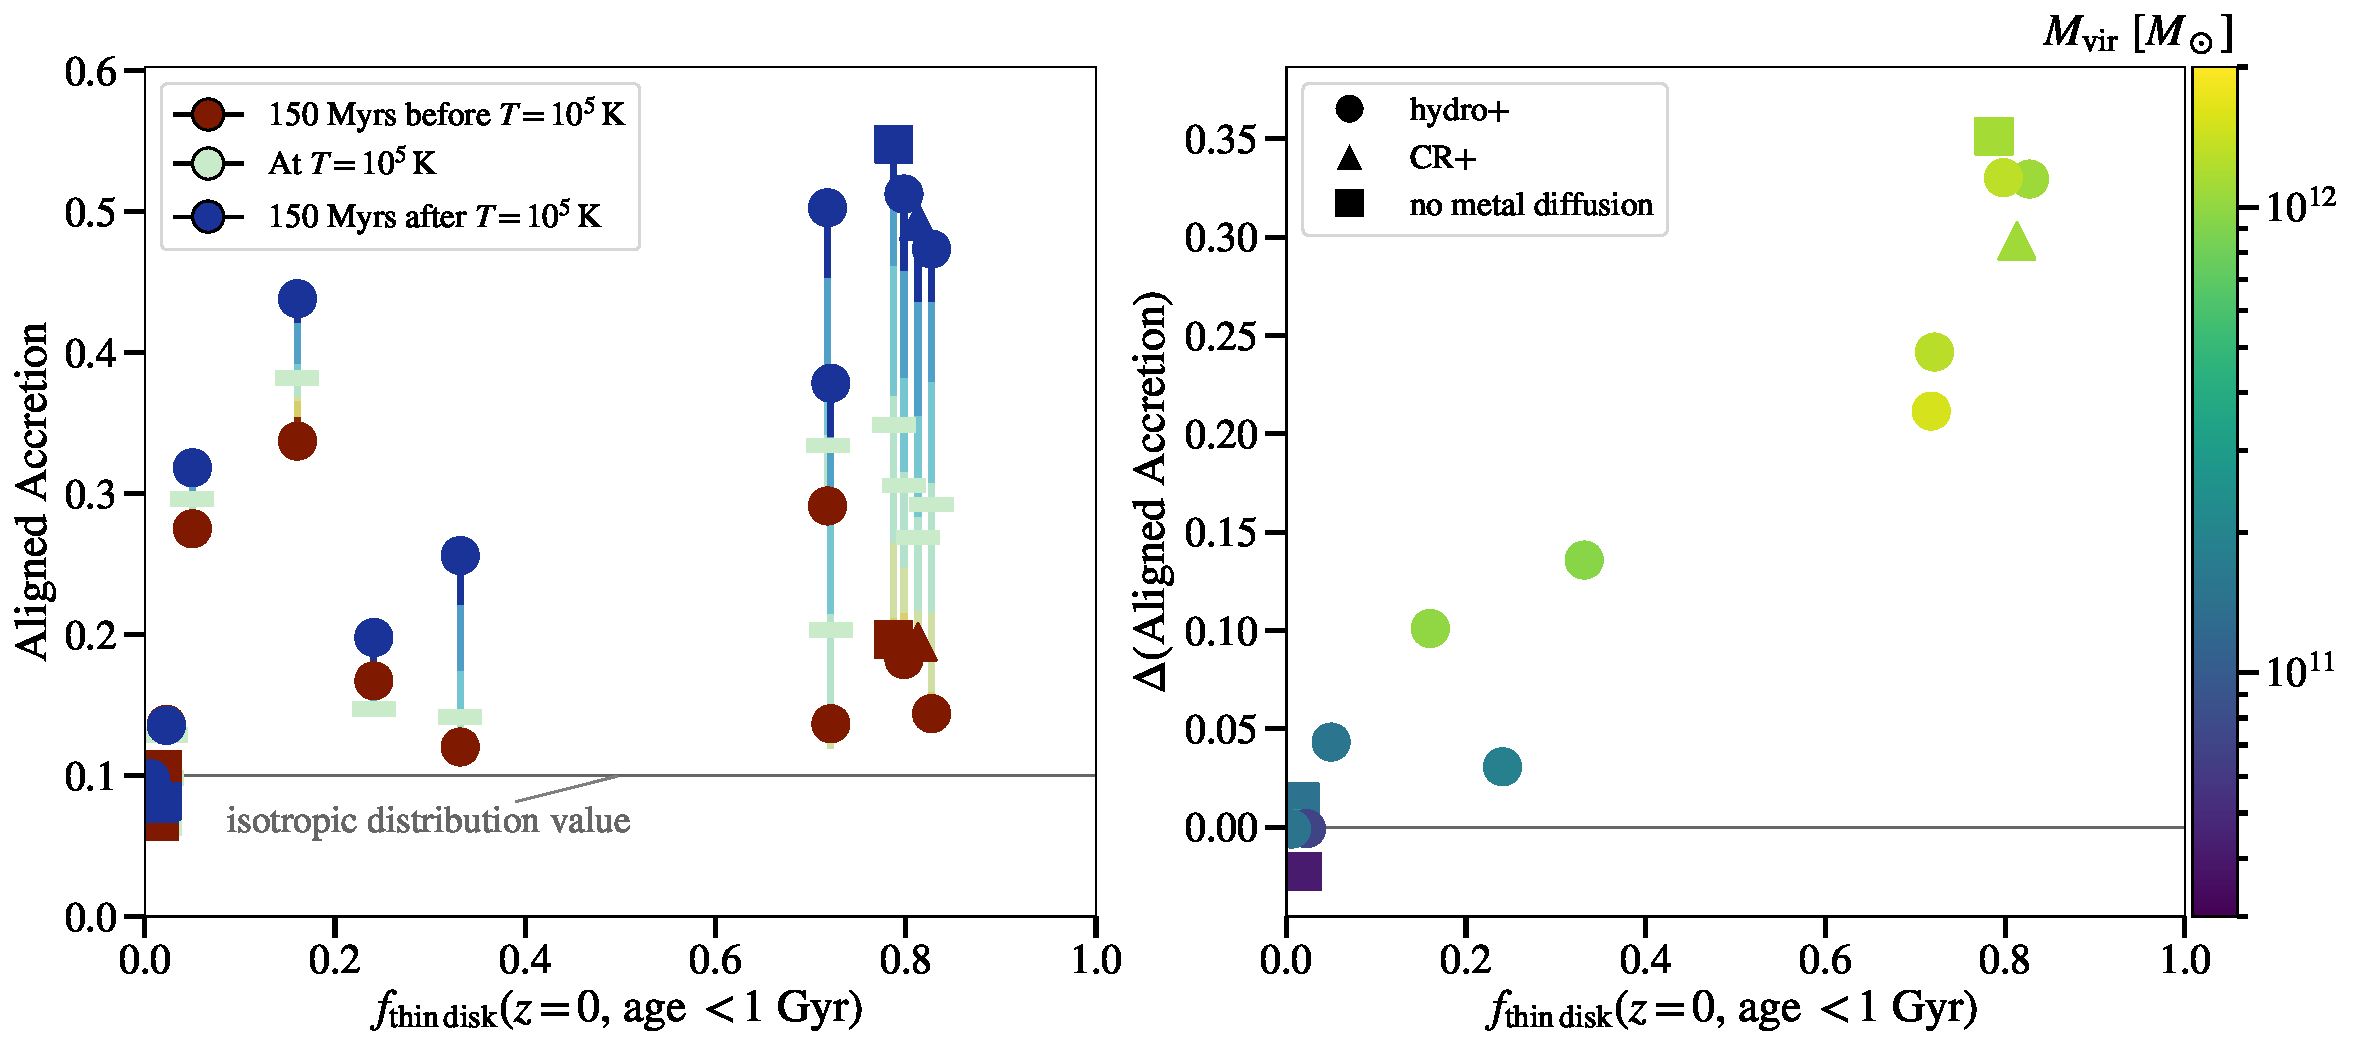
\includegraphics[width=\textwidth]{figures/prevalence/aligned_fraction.pdf}
    \caption{
    \textbf{Left:}
    Mass fraction of accreting gas aligned with the disc ($\vert z/R < 0.1 \vert$, see Fig.~\ref{f: theta vs t}) before and after cooling, for our sample of \Nsample~FIRE haloes.
    The horizontal axis plots the fraction of young stars in the central galaxy that are in a thin disc.
    \textbf{Right:}
    Change in aligned mass fraction during the $\pm200$ Myr around cooling time shown in the left panel.
    A large $\Delta f_{\rm aligned}$ indicates that circularization is concurrent with cooling.
    Color indicates virial mass.
    The value of $\Delta f_{\rm aligned}$ is strongly correlated with the fraction of young stars in a thin disc. %, regardless of halo mass.
    The square point that is circled on the right is \texttt{m12m}.
    This galaxy has developed a sizable secular bar at late times, which gives rise to a lower than expected thin disc fraction by our definition.
    }
    \label{f: prevalence}
\end{figure*}


% Figure description
Figure~\ref{f: prevalence} extends the analysis in Fig.~\ref{f: theta vs t} to the full sample.
We parametrize the extent to which flattening and cooling are concurrent via a parameter $f_{\rm aligned}$ (for ``spatial aligned accretion''), which corresponds to the fraction of accreting gas mass aligned with the disc plane ($\vert z/R \vert < 0.1$, marked by dashed vertical lines in Fig.~\ref{f: theta vs t}).
This range of angles contains $\approx 60\%$ of stars in thin discs~(by `thin disc' we mean stars with $j_z/j_c > 0.8$).
The left panel of Fig.~\ref{f: prevalence} shows the evolution of $f_{\rm aligned}$ from 200 Myr before $\tcools$ (red) to 200 Myr after $\tcools$ (blue), while the right panel shows the difference in $f_{\rm aligned}$ between these two epochs.
The horizontal axes plot the fraction of young stars in a thin disc $f_{\rm thin\,disc,\,recent}$. 
For most haloes the accreting gas is largely unaligned prior to cooling, with aligned mass fractions $f_{\rm aligned}\sim 0.1 - 0.2$ comparable to $f_{\rm aligned} = 0.1$ expected for an isotropic distribution.
Upon cooling, the alignment of accreting gas sharply increases in haloes with $f_{\rm thin\,disc,\,recent} > 0.5$ --- in most cases $\gtrsim 50\%$ of mass collapses to $\vert z/R \vert < 0.1$ during this time.
In contrast, in haloes with $f_{\rm thin\,disc,\,recent} \approx 0$ there is practically no change in $f_{\rm aligned}$ upon cooling.
Intermediate cases with $f_{\rm thin\,disc,\,recent} \approx 0.2-0.4$ typically show a modest increase in $f_{\rm aligned}$ and are further discussed in appendix~\ref{s: appendix-individual}.
The right panel of Fig.~\ref{f: prevalence} demonstrates the strong correlation between the change in $f_{\rm aligned}$ when the gas cools and the fraction of young stars in a thin disc. The halo circled in the right panel, \texttt{m12m}, is of special note:
gas accretes onto the halo as a rotating cooling flow, but subsequent evolution in the ISM and/or stellar population produces a stellar bar~\citep{Debattista2019}.
Fig.~\ref{f: prevalence} thus demonstrates, for our entire FIRE sample, that circularization is concurrent with cooling in accretion onto thin-disc galaxies, while no such association exists for accretion onto irregular or thick disc galaxies.

% MECHANICS OF QUIET ACCRETION
\begin{figure*}
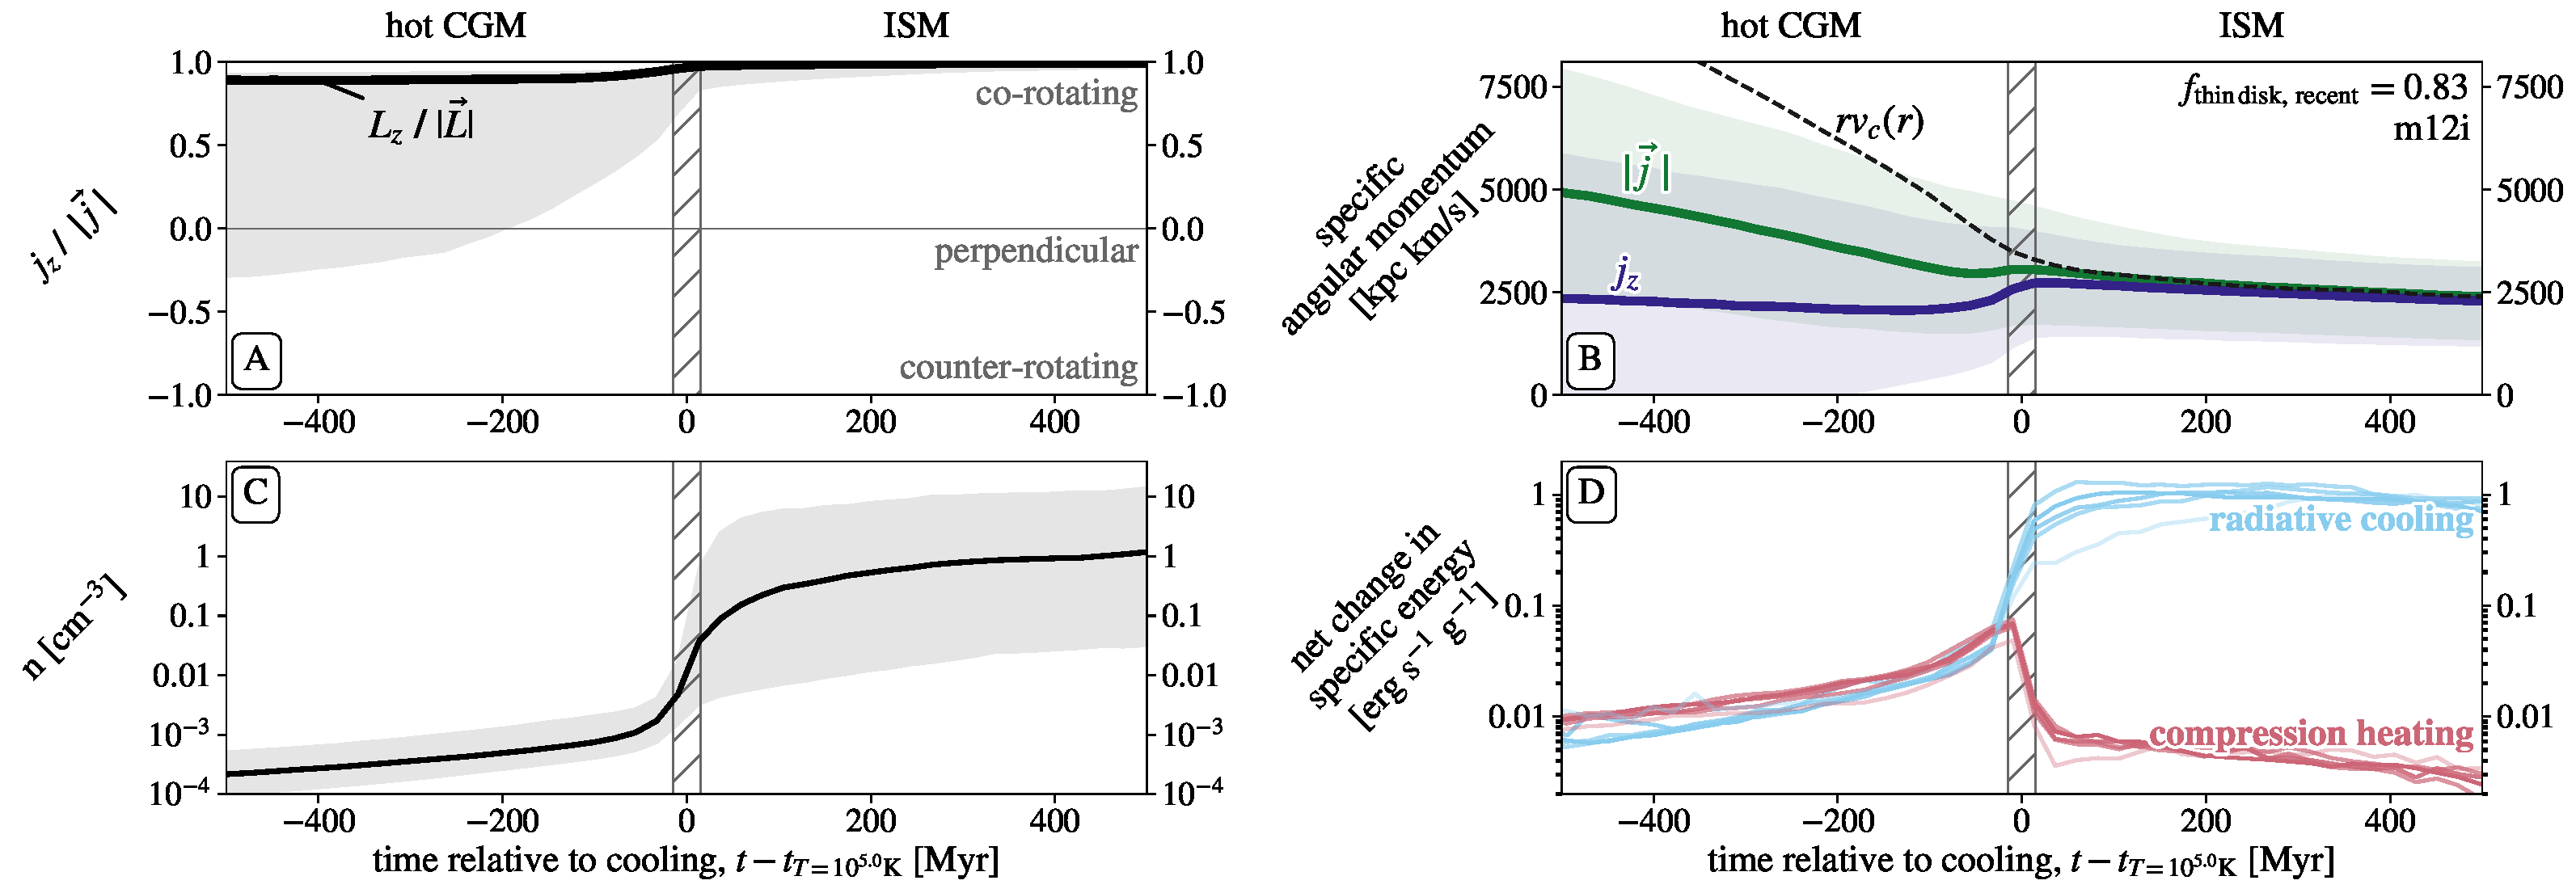
\includegraphics[width=\textwidth]{figures/before_and_after/before_and_after_m12i_md.pdf}
\caption{
Angular momentum and energetics of gas accreting onto the same $z\sim0$ thin disc galaxy shown in Fig.~\ref{f: before and after A}, versus time relative to the final cooling time ($t - \tcools$).
In each panel solid lines and shaded regions mark the medians and 16th to 84th percentile ranges of all particles accreted within 1 Gyr prior to $z=0$.
\textbf{A:}
The ratio of $j_z / \vert \vec j \vert$.
In only this panel the solid line shows this ratio for the sum total angular momentum of all accreted particles.
The shaded region shrinks as gas flows inward, indicating the flow becomes more coherent and that angular momentum unaligned with the total angular momentum is cancelled out, as suggested by Fig.~\ref{f: coherence}. 
\textbf{B:}
The magnitude of the specific angular momentum of particles ($\vert\vec{j}\vert$, green) and the component of angular momentum aligned with the galaxy disc ($j_z$; purple).
The dashed line shows the angular momentum necessary for rotational support.
Cooling occurs when angular momentum support becomes significant, as expected in subsonic cooling flows \citep{Cowie1980, Stern2019}.
\textbf{C:}
Baryon number density.
Prior to cooling the gas density increases due to the inflow.
As the gas cools the density sharply increases, due to the stalling of the inflow at the galaxy scale and the collapse into a disc geometry. 
\textbf{D:}
Energy loss from radiative cooling (blue) and heating from $PdV$ work on the gas particles (red).
Prior to cooling, compression heating offsets radiative cooling yielding the flat temperature profile seen in Fig.~\ref{f: before and after A}, as expected in a cooling flow.
Compression heating plummets after the inflow is stalled by angular momentum support.
\textbf{Change $Rv_c(R)$ to lowercase.}
}
\label{f: before and after B}
\end{figure*}

 % PREVALENCE OF QUIET ACCRETION - BEFORE/AFTER OVERVIEW
\begin{figure}
    \centering
    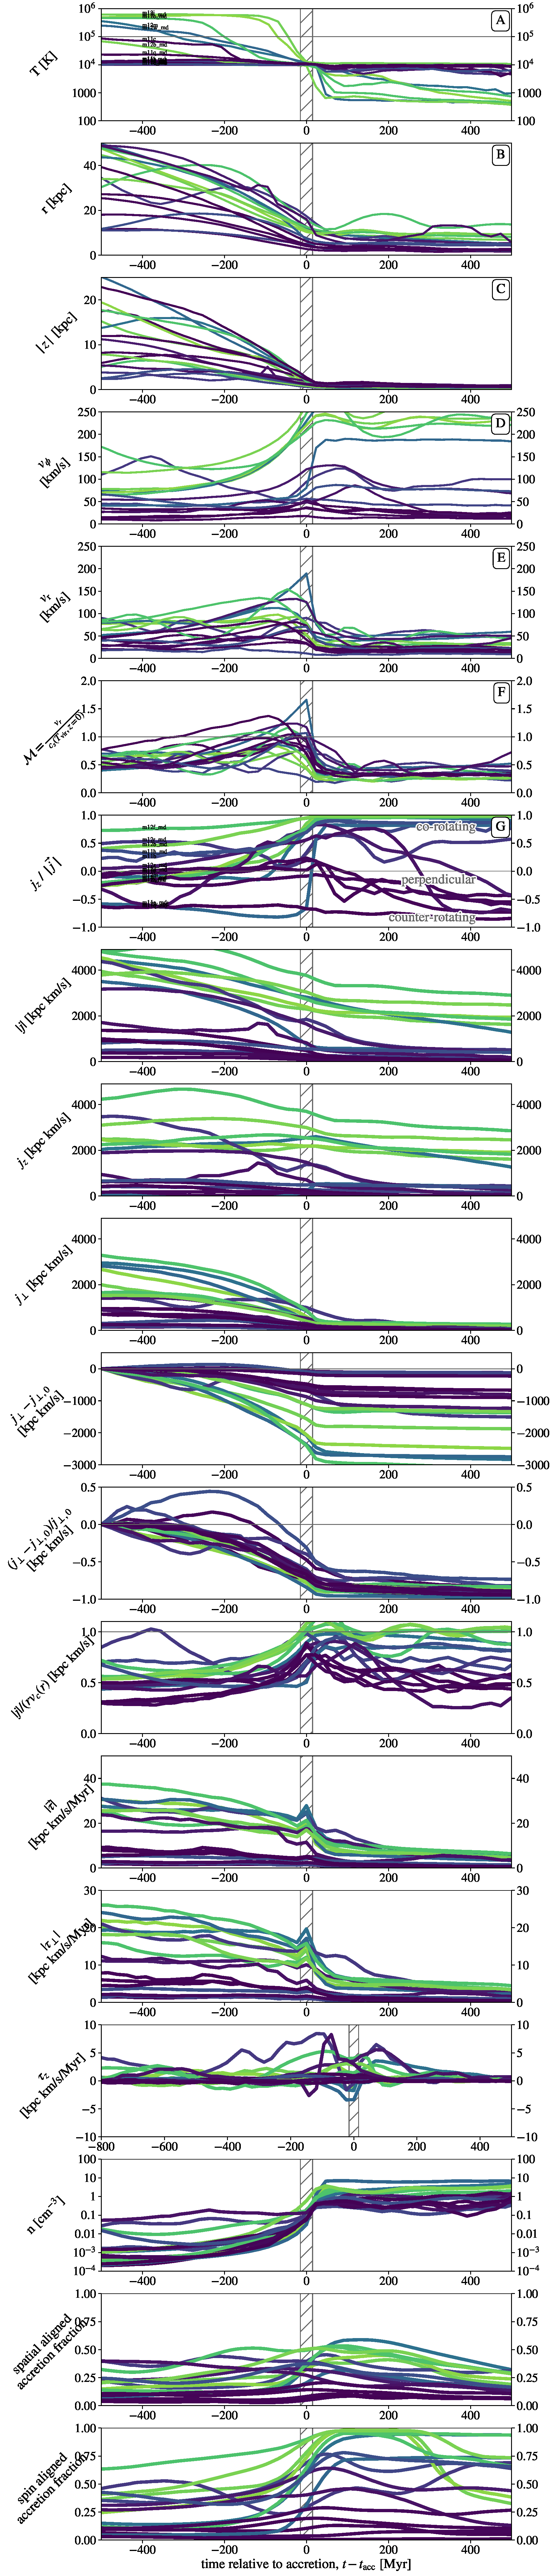
\includegraphics[width=\columnwidth]{figures/variations/relative_to_accretion/before_and_after/before_and_after_combined.pdf}
    \caption{
    Average properties relative to time of accretion for thin disk galaxies (orange; $f_{\rm thin\,disk}<0.5$) and irregular galaxies (purple; $f_{\rm thin\,disk}<0.5$).
    Solid line is the median of the solid line among thin disk/irregular galaxies, and the shaded regions cover the medians of the 16th to 84th percentile regions among thin disk/irregular galaxies.
    }
    \label{f: before and after - combined}
\end{figure}


% COHERENCE EVOLUTION
\begin{figure*}
    \centering
    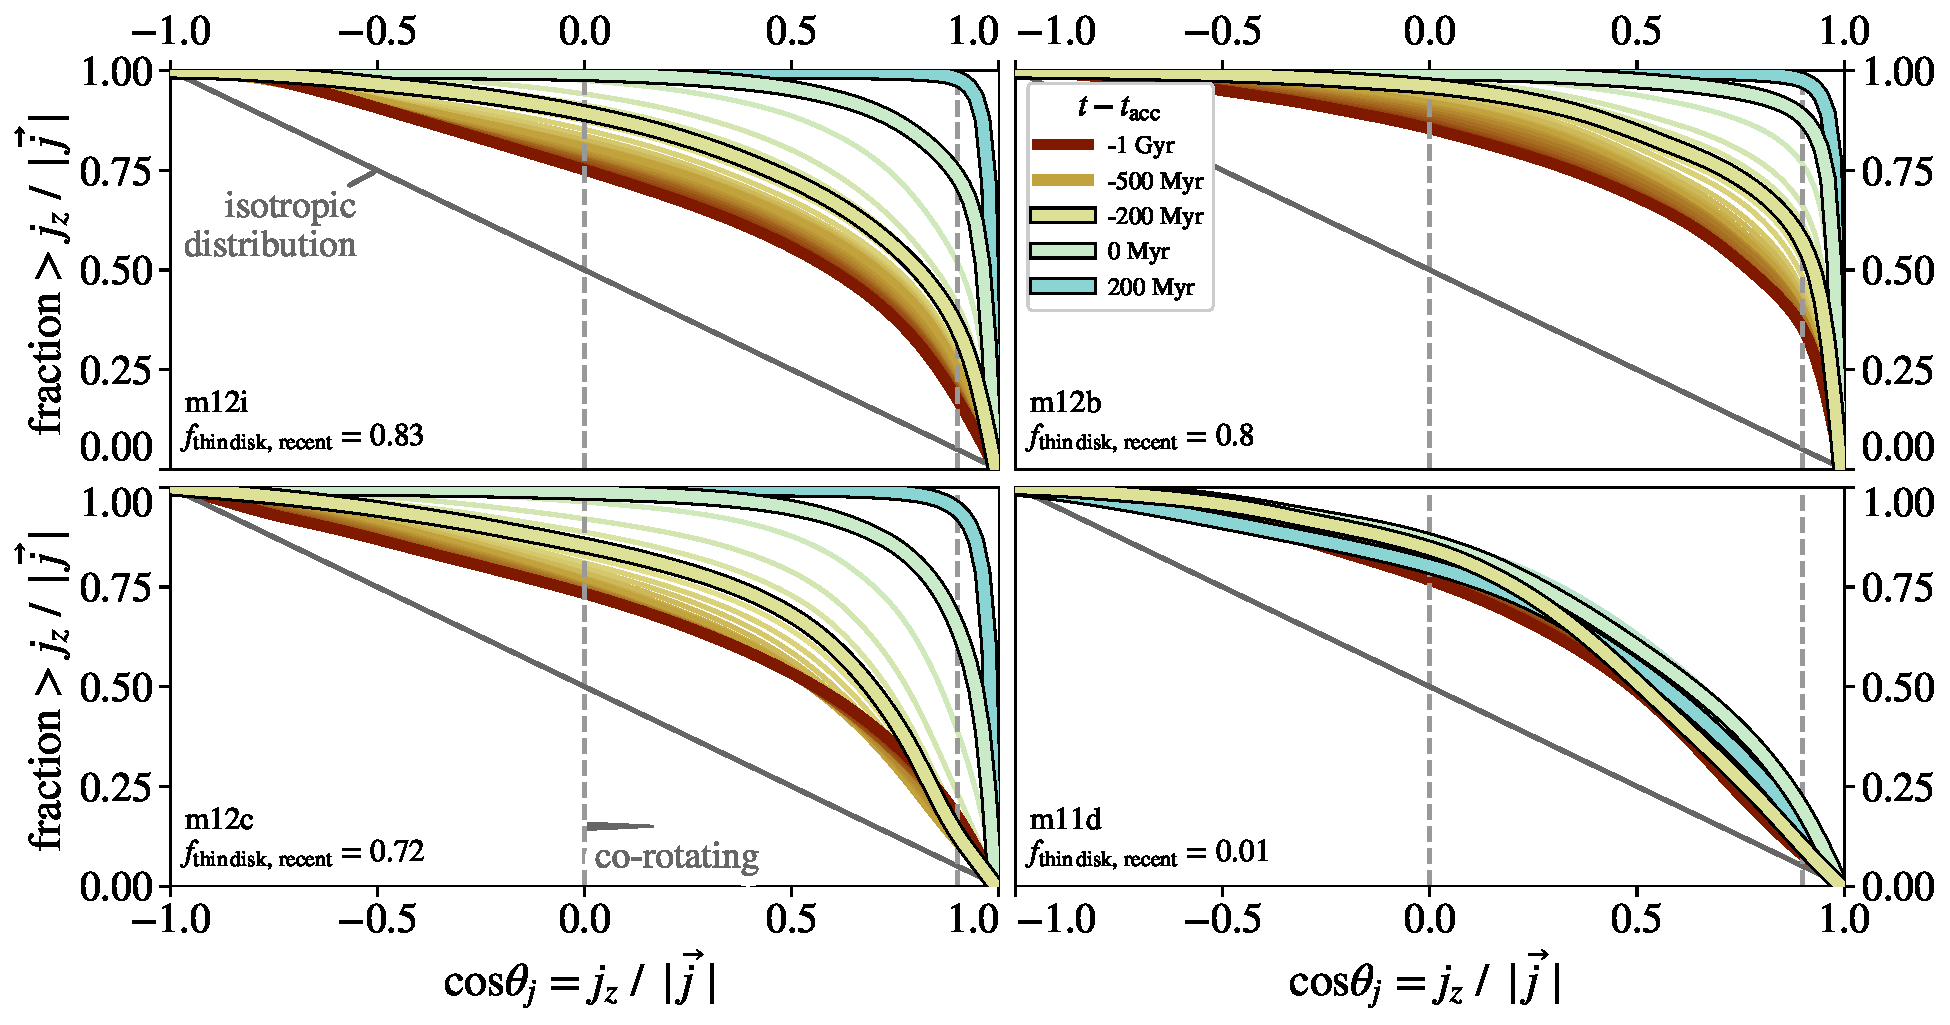
\includegraphics[width=\textwidth]{figures/variations/relative_to_accretion/jzjmag_vs_t.pdf}
    \caption{
    Angular momentum distribution of accreting gas, as a function of time relative to the last cooling time.
    Curves show the fraction of mass above a given $j_z / \vert \vec j \vert$. 
    In the thin-disc galaxies (top and bottom-left panels) the angular momentum distribution becomes more coherent and aligned with the central galaxy with time, mainly during the $\pm200$ Myr around the time of cooling.
    In the irregular galaxy (bottom right) the angular momentum distribution is quasi-spherical both before and after cooling. 
    }
    \label{f: coherence}
\end{figure*}

% PREVALENCE OF QUIET ACCRETION - ANGULAR MOMENTUM SPACE
\begin{figure*}
    \centering
    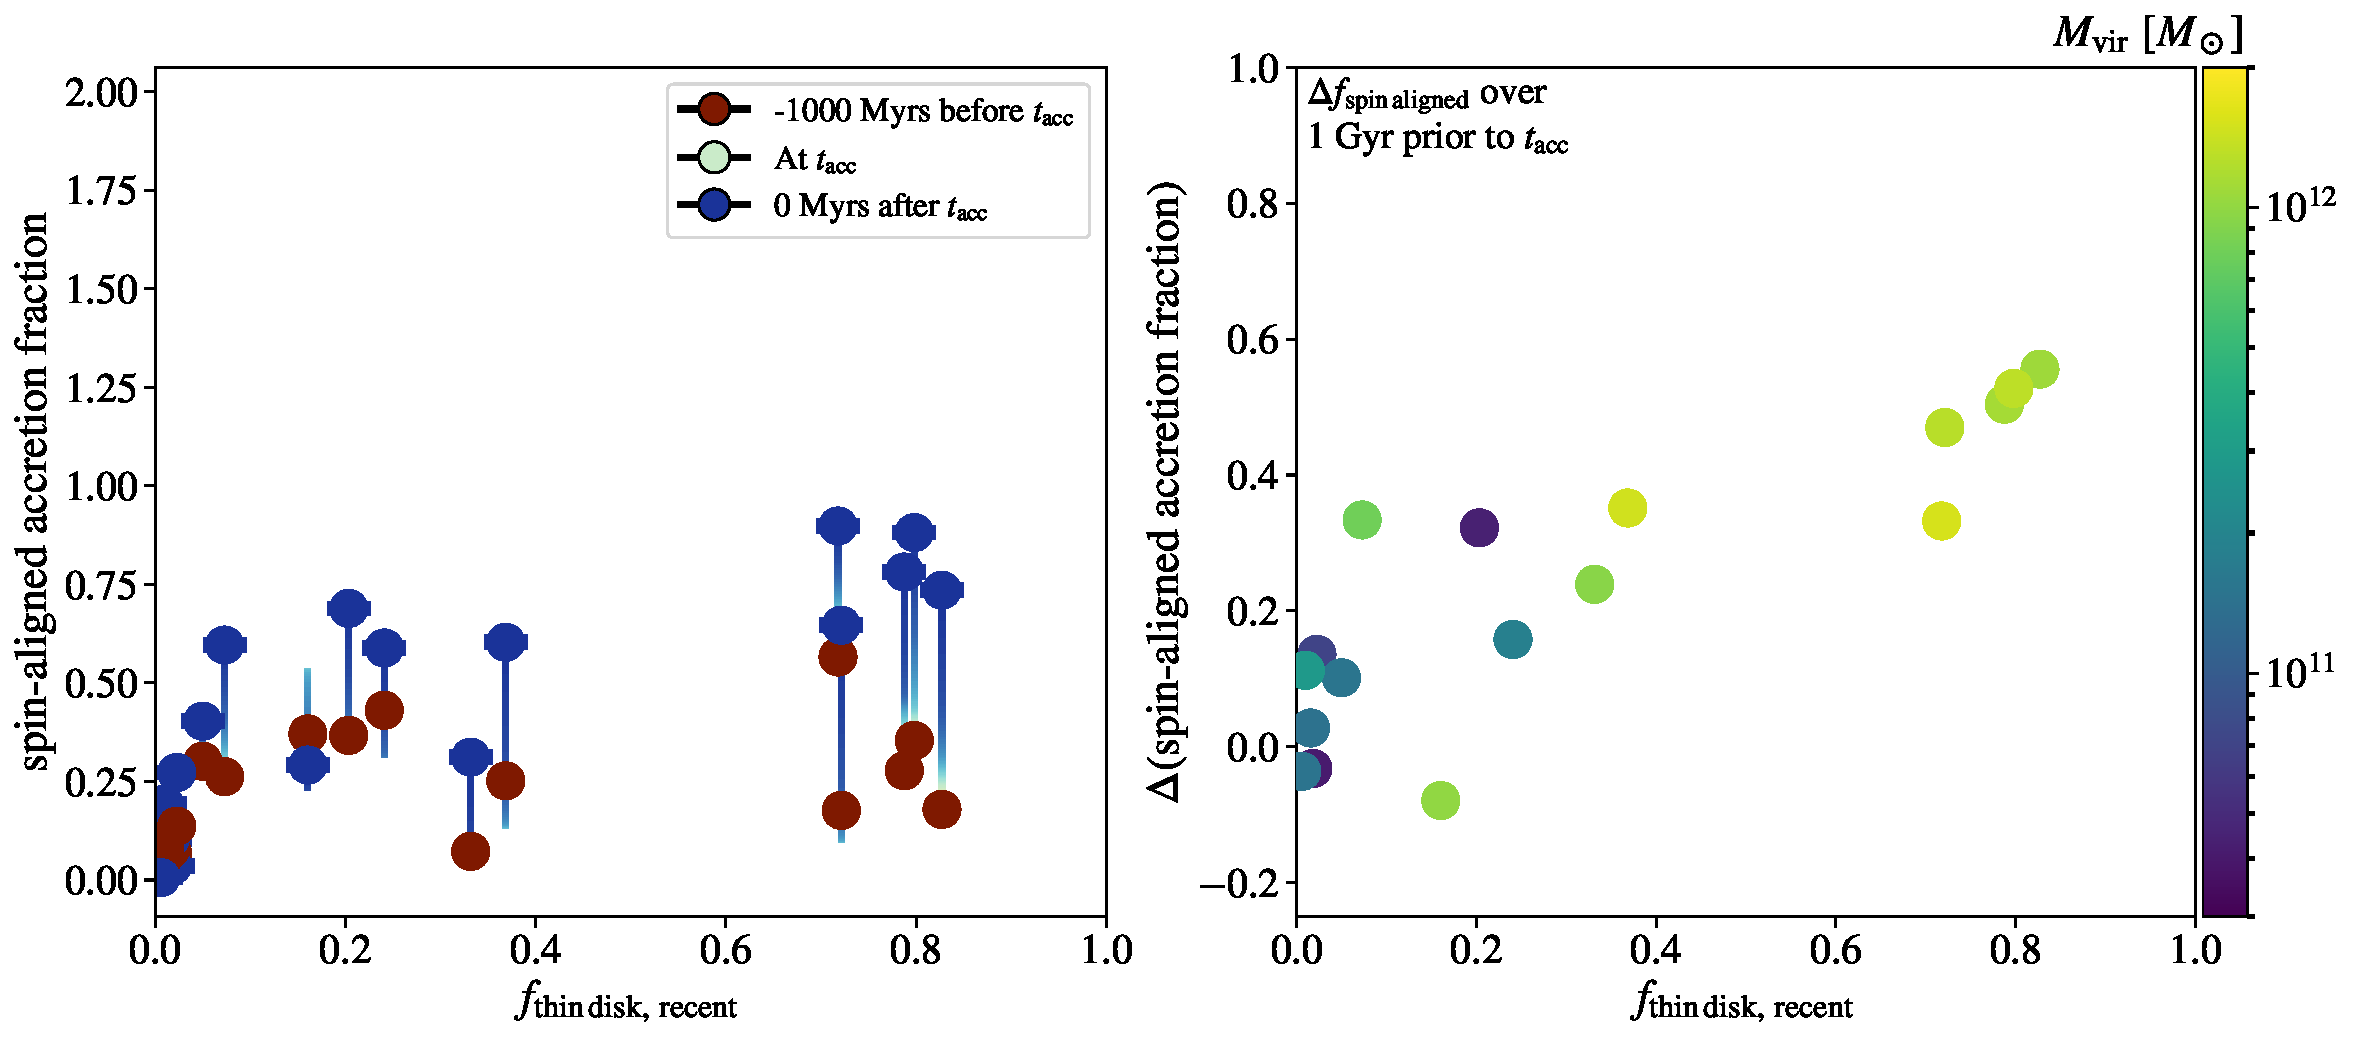
\includegraphics[width=\textwidth]{figures/variations/relative_to_accretion/prevalence/aligned_fraction_ang_momentum.pdf}
    \caption{
    Angular momentum-space equivalent of Fig.~\ref{f: prevalence}.
    \textbf{Left:}
    Mass fraction of accreting gas aligned with the disc before and after cooling, defined in this figure as the fraction with $\vert j_z/\vert j \vert > 0.9$ (see Fig.~\ref{f: coherence}).
    \textbf{Right:}
    Change in aligned mass fraction during the $\pm200$ Myr around cooling time shown in the left panel.
    The greater the extent to which accretion becomes coherent as it cools, the greater the fraction of young stars in a thin disc.
    }
    \label{f: prevalence - angular momentum}
\end{figure*}

\subsection{Angular momentum coherence in accreted gas}
\label{s: mechanics -- coherence}

% Figure coherence description
Figure~\ref{f: coherence} shows the cumulative distribution function of $j_z / \vert \vec j \vert$ in the accreted gas, weighted by mass, for the four simulations shown in Figure~\ref{f: theta vs t}.
This distribution quantifies the level of alignment of angular momentum in the accreted gas with respect to the rotation axis of the stars.
For reference, perfectly co-rotating gas has $j_z / \vert \vec j \vert = 1$, while perpendicular and counter-rotating gas have $j_z / \vert \vec j \vert = 0$ and $-1$, respectively.
An isotropic distribution of angular momentum would appear as a diagonal line in this plot. 
Each curve corresponds to a different range of $t - \tcools$ as noted in the legend. 
Outlined in black are the CDFs for the three times plotted in Fig.~\ref{f: prevalence}: $t - \tcools =$ -200, 0, 200 Myr.

% Overall evolution
In gas accreting onto thin disc galaxies (top and bottom-left panels of Fig.~\ref{f: coherence})  the angular momentum distribution becomes increasingly coherent with time relative to $\tcools$.
At $t-\tcools=-1$ Gyr the angular momentum distribution is marginally coherent, with only $\approx50\%$ of accreting gas co-rotating, with $j_z/\vert \vec j \vert > 0.5$.
In contrast at $t-\tcools=+500$ Myr the distribution is highly coherent, with $j_z/\vert \vec j \vert > 0.9$ for $\gtrsim 90\%$ of accretion.
The majority of the evolution in coherence occurs over $\lesssim 400$ Myr centered on $\tcools$, as seen by the differences between the outlined CDFs.
This increase in coherence allows the accreting gas to collapse into a thin disc as shown in Figs.~\ref{f: theta vs t}--\ref{f: prevalence}.
Furthermore, this result shows that accreting gas is almost entirely co-rotating with the galaxy {\em prior} to cooling, i.e., while the accretion is still part of the galactic `hot corona'. 
Close comparison with Fig.~\ref{f: theta vs t} shows that angular momentum coherence is achieved just prior to spatial flattening. 

In stark contrast with thin disc galaxies, the irregular galaxy \texttt{m11d} shown in the bottom-right panel of Fig.~\ref{f: coherence} experiences only a very mild evolution in angular momentum coherence --- angular momentum remains only marginally co-rotating both before and after cooling.

% Ang Momentum Prevalence
In Fig.~\ref{f: prevalence - angular momentum} we show the evolution of angular momentum alignment across the full sample, as Fig.~\ref{f: prevalence} did for spatial alignment. 
In this case, spin alignment is defined as the fraction of gas with $j_z/j > 0.9$.
As was the case for spatial alignment, a greater increase in spin alignment during cooling correlates with a greater thin disc presence.

% Coherence
The evolution of angular momentum in accretion onto thin discs is further explored in Figure~\ref{f: before and after B}, for the example case of \texttt{m12i}.
Panel (A) shows the median and 16th-84th percentiles in $j_z/\vert\vec j\vert$ for individual particles as a function of $t-\tcools$.
The dashed line plots this ratio for the {\em sum} of all particles at a given $t-\tcools$; the closer the dashed line and shaded region are, the more coherent the spin.
Note that the ratio of the total $j_z/\vert j \vert$ is not identically equal to unity because the $z$ direction is with respect to the central galaxy and {\em not} the gas itself.
Consistent with Fig.~\ref{f: coherence}, at $t-\tcools=-500$ Myr the ratio $j_z/\vert\vec j\vert$ spans a large range of $\approx -0.3 - 0.9$, while by $\tcools$ nearly all the accreting gas has $j_z\approx\vert\vec j\vert$, indicating all hot accreting gas particles are co-rotating.
On the other hand, the ratio $j_z/\vert\vec j\vert$ of the total angular momentum vector is nearly constant with time prior to accretion. 
These trends indicate that components unaligned with the net angular momentum are canceling out due to interaction in the hot halo.

% Support
Figure~\ref{f: before and after B} panel (B) shows the magnitude of the specific angular momentum ($\vert \vec j \vert$; green) and the z-component of the specific angular momentum ($j_z$; purple).
The median value $\vert \vec j \vert$ decreases prior to cooling, from $\approx 5000$ kpc km s$^{-1}$ to $\approx 3000\,{\rm kpc\,km\,s}^{-1}$, in contrast with  $j_z$ which remains constant.
The nearly constant $j_{\rm z}$ indicates the inflow conserves angular momentum in this direction, and is not subject to significant torques. 
The value of $j_z\approx 2500$ kpc km s$^{-1}$ is comparable to the average specific angular momentum of $j_{\rm DM} \simeq \sqrt{2}\lambda \Rvir \vvir$ expected in dark matter haloes due to tidal torques \citep[e.g.][]{Bullock2001}.
Using a typical dimensionless spin parameter $\lambda \simeq 0.035$, and the virial radius $\Rvir=270$ kpc and virial velocity $\vvir=130$ km s$^{-1}$ of this halo, we get $j_{\rm DM}\approx1750$ kpc km s$^{-1}$, i.e.~the expected average value of the dark matter is within $30\%$ of the net angular momentum of accreting hot gas shown in Fig.~\ref{f: before and after B}.~\footnote{The fact that the gas has slightly more angular momentum than naively expected for the dark matter is consistent with previous findings that gas typically has a slightly higher spin than dark matter \citep[e.g.][]{Stewart2017}.}

The dashed line in panel (B) of Fig.~\ref{f: before and after B} plots the median specific angular momentum necessary for gas to be fully supported by angular momentum at a given radius, i.e. $v_c(r)r$.
The accretion attains significant angular momentum support as it proceeds through the inner CGM, consistent with other analyses of CGM rotational support~\citep{Oppenheimer2018, Trapp2021}.
The values of $j_z$ and $v_c(r)r$ converge shortly after $t=\tcools$, indicating that cooling and a transition to rotational support occur almost simultaneously, as indicated also by Fig.~\ref{f: before and after A}.
This result is consistent with 1D steady-state cooling flow solutions which include angular momentum.
These solutions demonstrate that the hot inflow cools to $\sim10^4$ K at the radius where $j_z=r v_c(r)$, as long as the flow remains subsonic down to this radius \citep{Cowie1980, Stern2019}.

% The angular momentum increase
There is small but noticeable increase in $j_z$ at $t \approx \tcools$.
This increase is not the focus of our analysis, but we note that it may be a result of a difference in orientation and/or amplitude between the angular momentum of the galaxy and the angular momentum of the accreting gas~\citep[e.g.][]{Danovich2012, DeFelippis2017}, which forces the accreting gas to co-rotate with the galaxy.
The explicit mechanism to increase $j_z$ may be exchange of angular momentum via gravitational torques~\citep[e.g.][]{Danovich2015, Angles-Alcazar2021} or via collisional interactions.
Any angular momentum gained is expected to be lost by other particles, driving inflow of existing gas particles in the galaxy or galaxy-halo interface~\citep[e.g.][]{Mayor1981, Pezzulli2017}.
We note that the median increase in $j_z$ upon accretion and cooling shown in Fig.~\ref{f: before and after B} is quantitatively consistent with the observed $30\%$ difference between the rotation velocity of the the Milky Way disc and its hot CGM \citep{Hodges-Kluck2016}.

\subsection{Energetics of accreting gas}
\label{s: mechanics -- energy balance}
\textbf{Move section up.}

% Density
Figure~\ref{f: before and after B} panel (C) shows the distribution of the accreting gas density  versus time relative to cooling.
Prior to cooling the gas density increases steadily due to the inflow, reaching $\approx10^{-3}$ cm$^{-3}$ just before cooling at $t\lesssim\tcools$.
This density is comparable to observational estimates of the hot gas density just outside the Milky Way disc (e.g.,~\citealt{Li2017a}).
At $t\approx\tcools$, the gas density sharply increases, reaching $0.1$ cm$^{-3}$ within $\approx50$ Myr, due to the deceleration induced by the stalling of the inflow upon accretion (Fig.~\ref{f: before and after A}), and due to the collapse from a quasi-spherical geometry into a disc geometry. 

% Energy balance description
In Figure~\ref{f: before and after B} panel (D) we assess the energetics of the gas to determine why it cools.
We study the energetics through two types of change in specific energy: radiative cooling (blue lines) and compression heating (red lines).
Radiative cooling per unit mass for an individual particle is calculated as $\nH^2 \Lambda / \rho$, where $\nH$ is the hydrogen density, $\rho$ is the mass density, and $\Lambda$ is the cooling function for photoionized gas, which we take from \cite{Wiersma2009a}.
Compression heating per unit mass for an individual MFM resolution element is calculated as $P \frac{dV}{dt} \approx \frac{ P }{ n^2 } \frac{ \Delta n }{ \Delta t }$, where $P = n k_B T$, $\Delta \rho$ is the change in density from one snapshot to the next, and $\Delta t$ is the snapshot time spacing.
Because accreting gas elements interact with other accreting gas elements thermodynamically we show the mean specific energy tracks of all gas elements binned into 100 Myr bins of $\tcools$.
To focus on the behavior of the majority of the particles we do not bin the $1\%$ of particles with the highest change in specific energy.
Some $\tcools$ bins contain much more accreting gas than others, and to reflect this we set the darkness of the lines proportional to the number of particles in the bin.

% Energy balance trend
At $t-\tcools=-500$ Myr the radiative cooling rate is $\approx0.006$ erg s$^{-1}$ g$^{-1}$, corresponding to a cooling time of $400$ Myr for the median temperature of $T=4\times 10^5$ K at this epoch (see Fig.~\ref{f: before and after A}, panel A).
At $t-\tcools =-500$ Myr the cooling time is thus comparable to the accretion time of $\approx500$ Myr.
At later $t-\tcools$ but still prior to cooling, the radiative cooling rate increases due to the increase in gas density.
The panel however shows that this energy loss to radiation  is nearly completely offset by compressive heating, explaining the roughly flat temperature profile at $t<\tcools$ (Fig.~\ref{f: before and after A}). 
These equalities between the cooling time and the accretion time, and between radiative cooling and compressive heating, are defining characteristics of classic cooling flows in which angular momentum support can be neglected \citep{Mathews1978, McNamara2007, Stern2019}. 

Around $\tcools$ the cooling rate and compressive heating diverge.
This can be understood by noting that the radiative cooling rate per unit mass scales as $\propto\rho\Lambda$, while the compressive heating rate scales as $\propto\epsilon d\log\rho/d t$ where $\epsilon$ is the specific thermal energy.
The deceleration of the hot inflow prior to accretion onto the galaxy causes $\rho$ to increase faster than $d\log\rho/d t$, causing the temperature to decrease.
This in turn increases the cooling rate and decreases $\epsilon$, which further accelerates the drop in temperature.
The result is gas that cools from $\approx10^6$ K to $\approx10^4$ K over the course of $\lesssim 50$ Myr.

\section{Discussion}
\label{s: discussion}

In this paper we analyse the properties of gas accreting onto $z\sim0$ galaxies simulated in FIRE, focusing on Milky-Way mass galaxies in which new stars form in a thin disc. 
We find that thin disc galaxies in FIRE accrete via `rotating cooling flows', a mode of `hot accretion' in which the quasi-spherical $T\sim\Tvir$ CGM phase inflows towards the galaxy, remaining hot down to the radius where its angular momentum is sufficient to provide rotational support.
At this radius ($\gtrsim 4 r_{\star,0.5}$, just outside the galaxy radius) the hot inflow both decelerates and becomes coherently rotating, and then simultaneously cools and collapses into a rotating cool disc.
Our results thus extend classic cooling flow theory by demonstrating their applicability in realistic cosmological simulations, and by exploring the mechanics of cooling flows with angular momentum, a subject which has not yet been studied extensively~\citep[c.f.][]{Cowie1980, Stern2019}.
Moreover, we find a strong correlation between the prevalence of this accretion mode and the fraction of stars in the central galaxies that form in a thin disc, potentially indicating that a rotating cooling flow is a necessary condition for the formation of a thin star-forming disc.
In this section we discuss several interpretations, caveats, and implications of our results. 

\subsection{Why are rotating cooling flows conducive to thin disc formation?}
\label{s: why CFs thin discs}

Our analysis identifies two properties of rotating cooling flows that likely promote the formation of thin star forming discs in the central galaxy.
These include the tendency of rotating cooling flows to become coherently rotating \textit{prior} to cooling and accretion onto the galaxy (Fig.~\ref{f: coherence} and panels A--B in Fig.~\ref{f: before and after B}),
and their tendency to decelerate \textit{before} accretion (panel D in Fig.~\ref{f: before and after A}).
Combined, these two properties indicate that upon cooling the accretion flow forms a thin disc with $v_\phi\approx v_{\rm c}$ and $v_r, v_z \ll v_{\rm c}$. 
Though any accreting collisional medium is expected to eventually equilibriate into such a coherently rotating disc, in rotating cooling flows this coherence is achieved \textit{prior} to cooling and accretion onto the ISM.
This both implies that the accretion process does not stir turbulence in the ISM efficiently (in contrast with cold streams as discussed in \citealt{Dekel2009}), and that star formation commences only after the accreting gas forms a thin gaseous disc morphology (Fig.~\ref{f: before and after A}).
In contrast, in other accretion modes some stars may succeed in forming while the accreting gas morphology is still a thick disc or irregular.
Such stars will inject feedback momentum and energy into their surroundings which could further delay the equilibration process, allowing even more stars to form outside of a thin disc. 

Why do hot inflows decelerate and rotate coherently prior to accretion?
We argue here that these characteristics are a result of the subsonic nature of the flow, though defer a formal derivation to future work. 
In a subsonic flow gradual deceleration prior to accretion is expected since the inflow is `forewarned' (via changes in pressure) of the transition to rotational support at the galaxy scale.
This is in contrast with supersonic accretion modes where the accreting gas is expected to shock and halt abruptly at the galaxy scale.
The subsonic nature of hot inflows may also induce the angular momentum coherence achieved near the rotational support radius (Fig.~\ref{f: before and after B}, panel A).
This follows since at the rotational support radius the mean rotational velocity $\langle v_\phi \rangle$ is approximately the circular velocity (neglecting radial pressure gradients; e.g. \citealt{Wellons2020}), while $v_{\rm c}^2\approx c_{\rm s}^2$ in hot flows, where $c_{\rm s}$ is the sound speed.
Thus, the mean Mach number in the $\phi$ direction approaches unity at the rotational support radius, and order unity velocity fluctuations around this mean would lead to speeds which approach or exceed the sound speed.
Since such supersonic fluctuations will rapidly shock and convert their kinetic energy into thermal energy, we expect any velocity fluctuations induced by a broad distribution of angular momentum to rapidly fade out when the hot flow approaches the rotational support radius, yielding a coherent accretion flow.

\subsection{When and where do we expect thin discs?}

% PREVALENCE OF QUIET ACCRETION -- VS GALAXY PROPERTIES
\begin{figure*}
    \centering
    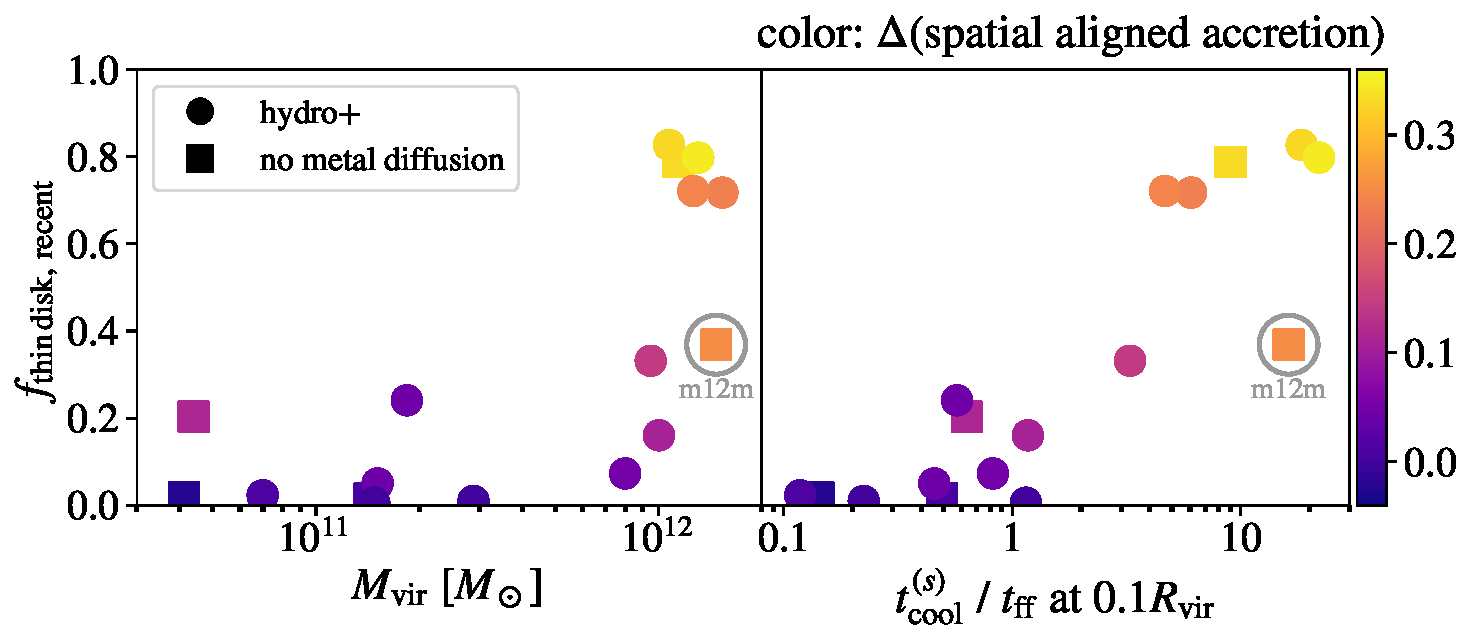
\includegraphics[width=\textwidth]{figures/prevalence/aligned_fraction_vs_galaxy_props.pdf}
    \caption{
    Fraction of young stars in a thin disc versus $M_{\rm vir}$ and $t_{\rm cool}^{(s)}/t_{\rm ff}$ evaluated at $0.1 R_{\rm vir}$.
    Color indicates change in the fraction of accreted gas which is aligned with the central galaxy, during $-200\,{\rm Myr} < t-\tcools < 200\,{\rm Myr}$ (see Fig.~\ref{f: prevalence}).
    For $M_{\rm vir} < 10^{12} M_\odot$ both the thin disc fraction and $\Delta f_{\rm aligned}$ are small.
    In more massive galaxies these quantities span a large range.
    The square point that is circled on the right is \texttt{m12m}.
    This galaxy has developed a sizable secular bar at late times, which gives rise to fairly low thin-disc fraction by our definition. 
    }
    \label{f: prevalence vs galaxy properties}
\end{figure*}

\newcommand{\tcoolsh}{t_{\rm cool}^{(s)}}
\newcommand{\tff}{t_{\rm ff}}
\newcommand{\Mvir}{M_{\rm vir}}


The scenario suggested by this paper, \textit{that thin star forming discs are a result of accretion via rotating cooling flows}, allows us to predict at which halo masses and redshifts we expect thin discs to form (although we caution that our preceding analysis focused on $z\sim 0$).
Cooling flows are expected only following the formation of a time-steady and pressure-supported `virialized CGM', which occurs when the cooling time of hot shocked CGM gas $\tcoolsh$ exceeds the free-fall time $\tff$ at halo masses above a threshold of $\sim10^{11}-10^{12}\msun$ \citep{White1978, White1991, Birnboim2003}. 
We note that by virialized CGM, we refer to the volume-filling phase.
In particular, a volume-filling cooling flow can co-exist with cold streams, especially at $z>1$ \cite[e.g.,][]{Keres2005,Dekel2006, Dekel2009}.
We must also consider the fact that a cooling flow could be disrupted by heating from feedback as envisioned in `thermal-balance'  models of the CGM \citep[e.g.,][]{Mccourt2012, Sharma2012, Voit2017, Faerman2017, Faerman2020}.
Furthermore, \cite{Stern2019} demonstrated that even if a virialized CGM exists in the outer halo and heating by feedback can be neglected, the resulting cooling flow may go through a sonic point and reach the galaxy as cool supersonic accretion.
Thus, to produce cooling flows that remain hot and subsonic down to the galaxy scale as found above for thin disc galaxies, a more specific condition should be satisfied, namely that $\tcoolsh$ exceeds $\tff$ at an inner CGM radius of $\approx0.1 r_{\rm vir}$.
In our simulation sample, this latter condition is met and the inner CGM indeed virializes at $\Mvir\approx10^{12}\msun$, roughly independent of redshift (\citealt{Stern2021}), although in the case of baryon-depleted, metal-poor, or high-spin galaxies inner CGM virialization can occur at a lower mass.

Figure~\ref{f: prevalence vs galaxy properties} shows the relationship between thin disc fraction and virial mass (left panel), and $\tcoolsh/\tff$ at $0.1 r_{\rm vir}$ (right panel), in our sample of $z\sim0$ FIRE galaxies.
Markers are colored by $\Delta f_{\rm aligned}$, a measure of the dominance of rotating cooling flows in accreting gas (Fig.~\ref{f: prevalence}).
The figure shows that thin discs and rotating cooling flows appear at $M_{\rm vir}\approx 10^{12}\msun$ and $\tcoolsh/\tff(0.1\Rvir)>1$, consistent with the expectation noted above that cooling flows and hence thin discs commence only when the inner CGM virializes.
This mass scale for thin disc formation is however larger than in $z\sim0$ observations, as further discussed in the next section.

% Necessary but not sufficient
We note that accretion via a rotating cooling flow does \textit{not} ensure a thin disc forms. 
A merger, a strong feedback event, or other disruptions may take a thin gaseous disc and disturb it, preventing stars from forming in a thin disc.
(Conversely, there is evidence that in many of the FIRE-2 MW-mass galaxies the disc orientation of many not be stabilized until after the last major merger~\citealt{Santistevan2021a}).
Simulation \texttt{m12m} provides evidence of this:
it has rotating cooling flow accretion comparable to thin disc galaxies ($\Delta f_{\rm aligned} \approx 0.25$), but has a relatively small $f_{\rm thin\,disc,\,recent} \approx 0.4$ (yellow square in Fig.~\ref{f: prevalence}).
However, the strong correlation seen in Fig.~\ref{f: prevalence} between the prevalence of rotating cooling flow accretion (quantified via $\Delta f_{\rm aligned}$) and the thin disc fraction $f_{\rm thin\,disc,\,recent}$ suggests that such events are relatively rare. 


The result in Fig.~\ref{f: prevalence vs galaxy properties} that cooling flows occur when $\tcoolsh>\tff$ at $0.1\Rvir$ and the inner CGM virializes indicates that any heating of the CGM by stellar feedback during the epoch of steady star formation in FIRE is insufficient to disrupt the cooling flow.
This is consistent with the weak outflows at this mass and redshift scale in the FIRE simulations \citep{Muratov2015, Muratov2017, Angles-Alcazar2017, Stern2021, Pandya2021} and in observations \citep[e.g.,][]{Heckman2019}.
The potential effects of AGN feedback, not implemented in the FIRE sample used in this work, are further discussed in \S~\ref{s: caveats}. 

How does thin disc formation depend on redshift?
While the threshold of inner CGM virialization is roughly independent of redshift, the importance of cold streams penetrating the hot halo is expected to be redshift-dependent, and thus if thin discs form as a result of hot accretion we expect them to be rarer at high redshift.
This expectation is realized in FIRE~\citep{Angles-Alcazar2017a, Ma2018, Wellons2020}, where discs that form following virialization at $z\gtrsim2$ tend to be thicker ($V_{\rm rot}/\sigma_z\approx2-3$, see fig.~14 in \citealt{Stern2021}) than their low-redshift counterparts discussed in this work ($V_{\rm rot}/\sigma_z\approx7-10$).
This trend is also qualitatively consistent with other simulations which show relatively thick discs at high redshift (e.g.,~\citealt{Pillepich2019, Dekel2019}) and with the thicker discs seen in high-redshift observations~\citep[e.g.][]{Tadaki2017}.

We note that while the thickness of massive discs and the dominance of cooling flows in FIRE appear to depend on redshift (this could be due, e.g., to evolving gas fractions $f_g$, since in equilibrium disc models the thickness of the disc scales with $f_g$;~\citealt{Thompson2005, Faucher-Giguere2013}), other transitions coincident with inner CGM virialization appear to be redshift-independent.
These include the suppression of stellar-driven outflows on CGM scales and the transition from rapidly fluctuating (`bursty') star formation to time-steady star formation (\citealt{Stern2021, Yu2021}, Gurvich et al., in prep).
These transitions may hence be tied more directly to a different effect of inner CGM virialization, such as the confinement of outflows by pressurized, hot gas (see \citealt{Stern2021}). 

\subsection{Analogous accretion in cosmic ray-dominated haloes}
\label{s: crs}

In Fig.~\ref{f: before and after m12i cr} in the appendix we plot the properties of accreting gas in a simulation that includes cosmic ray physics ~\citep[][]{Chan2019, Hopkins2020a}, thus providing a window into the differences in gas accretion modes in simulations with non-thermal support.
The accretion onto the central galaxy in this simulation (\texttt{m12i\_cr}) is similar to rotating cooling flows in many aspects:
accreting gas gains coherence in the halo, becomes rotationally supported at the galaxy edge (with a decreased radial velocity), and subsequently collapses into a disc.
These properties were highlighted also by \cite{Trapp2021}, who performed an analysis on the accretion of gas onto MW-mass disc galaxies with CR-dominated haloes.
Consistent with our results, \citeauthor{Trapp2021} found that accretion onto MW-mass discs has the same qualitative behavior, regardless of whether or not the halo is CR-dominated.
However, panels A and I of Fig.~\ref{f: before and after m12i cr} demonstrates that accreting gas in CR-dominated haloes never shocks to a temperature $T \sim T_{\rm vir} \sim 10^{5.5}$ K and the radiative cooling is not offset by compression heating, i.e. the accretion is not a cooling flow.
This is because \texttt{m12i\_cr} is dominated not by thermal pressure, but by cosmic ray (CR) pressure that provides support against gravity without significantly heating the gas~\citep{Ji2020}.

% Mechanics
Increased coherence and decreased radial velocity prior to accretion, the two properties of rotating cooling flows we identify as promoting thin disc formation (\S\ref{s: why CFs thin discs}), are clearly present in \texttt{m12i\_cr} (Fig.~\ref{f: before and after m12i cr}).
Consistent with this, \texttt{m12i\_cr} has a high thin disc fraction, $f_{\rm thin\,disc,\,recent}=0.71$.
In \S\ref{s: why CFs thin discs} we argue that the coherent co-rotation and deceleration of rotating cooling flows is a result of its subsonic nature.
Consistent with this, the accreting gas in the CR-dominated halo is also effectively subsonic, wherein 
gas elements interact via CR pressure rather than thermal pressure. 
The qualitatively similar behavior between both rotating cooling flows and accretion in CR-dominated haloes suggests these accretion modes are a subset of a more general form of \textit{disc-conducive subsonic accretion}.

\subsection{Caveats}
\label{s: caveats}

% Overprediction of star formation
In our MW-mass haloes the average SFR over $z=0-0.5$ is SFR$\approx 3-10\,M_\odot/$yr, while the observationally-based average SFR for $M_{\rm vir} \sim 10^{12} M_\odot$ haloes over the same redshift range is SFR$\approx 0.7-6\,M_\odot/$yr~\citep{Behroozi2013} (though Gandhi et al., in prep find that the SFR is consistent with other observational constraints).
Since one component that regulates the SFR is the gas accretion rate onto the galaxy, it is possible that our simulations have higher accretion rates from the CGM onto the galaxy $\Mdot_{\rm CGM}$ than in real galaxies at the same mass scale (although note that observational estimators do not fully capture SFR; \citealt{Velazquez2020}).

The CGM accretion rate may be reduced if the cooling flow is disrupted by additional physics implemented in some other suites of FIRE simulations, including cosmic rays~\citep{Chan2019, Hopkins2020a, Hopkins2021e, Hopkins2021d} and AGN feedback (Wellons et al. in prep.).
It is however unclear whether additional processes such as these can disrupt cooling flows around MW-way mass galaxies.
For example, CR transport models remain highly uncertain, especially in the CGM~\citep{Hopkins2021, Quataert2021, Quataert2021a}, and it is not yet known how AGN feedback couples to halo gas.
Moreover, if AGN feedback is intermittent, it is possible that a rotating cooling flow could reform between bursts of AGN feedback.

An alternative solution to the elevated accretion rate problem is that the cooling flow is not disrupted, but just weaker than in FIRE if the CGM mass or metallicity are overpredicted in FIRE at $z\sim0$.
This follows since in a cooling flow $\Mdot_{\rm CGM}\propto M_{\rm CGM}^2 \Lambda(Z)$, where $M_{\rm CGM}$ is the CGM mass and $\Lambda$ is the cooling function.
Thus, if the CGM mass is overpredicted by a factor of two then $\Mdot$ and the SFR would be overestimated by a factor of four.
Both the CGM mass and metallicity are a result of the integrated enrichment and depletion of the CGM by outflows over cosmic time, and thus are uncertain~\citep[e.g.,][]{Davies2021, Kelly2021}.
A lower CGM mass than found in FIRE would also be more consistent with several studies of X-ray emission from the MW which find $M_{\rm CGM}/f_bM_{\rm vir} \approx 0.1$~\citep[][]{Li2018, Bregman2018}, where $f_b M_{\rm halo}$ is the cosmological baryon fraction multiplied by the halo mass.
This is in contrast with $M_{\rm CGM}/f_bM_{\rm vir} \approx 0.2-0.4$ for similar-mass FIRE haloes~\citep{Hafen2019}, though note that other studies deduce $M_{\rm CGM}/f_bM_{\rm halo}=0.3$ based on the same X-ray data~\citep{Faerman2020}.
Note, however, that directly comparing mock X-ray emission to observations (with the same stellar mass or SFR) shows that FIRE haloes both with and without CRs are on the low end of observed emission, but may not be excluded~\citep{Chan2021}.

At $z\sim0$, FIRE galaxies only have significant significant rotational support ($V_{\rm rot}/\sigma_z > 1$) above $M_\star\sim10^{10}\msun$, in contrast with observations which find rotationally-supported galaxies above $M_\star\sim10^9\msun$ (\citealt{El-Badry2018a, El-Badry2018}, see also \citealt{Peebles2020}).
A lower CGM mass may help address this apparent difference.
This follows since a lower $M_{\rm CGM}$ both implies a lower SFR and hence lower $M_\star$ for a given halo mass, and a lower halo mass threshold for inner CGM virialization, since $\tcoolsh$ is larger when $M_{\rm CGM}$ is lower. 
The latter effect would cause the onset of cooling flows and the formation of thin discs to occur at lower halo masses than suggested by Fig.~\ref{f: prevalence vs galaxy properties}.
\cite{Stern2021} showed that at $z\sim0$ a factor of a few increase in $\tcoolsh$ relative to that in FIRE would decrease the threshold halo mass in which the inner CGM virializes to $M_{\rm vir}\sim10^{11}\msun$, corresponding to a threshold stellar mass of $M_\star\sim10^9\msun$ for thin disc formation.

\subsection{Comparison to observations}
\label{s: discussion -- observations}

\cite{Hodges-Kluck2016} analysed the velocity shifts of O{\sc VII} absorption lines originating in the Milky-Way halo, observed with XMM-Newton towards an ensemble of AGN. 
They deduced that the hot inner CGM of the Milky Way (or `Galactic corona') is rotating at $180\pm40$ km s$^{-1}$, corresponding to $60-90\%$ of the rotation velocity of the disc.
This result is consistent with a rotating cooling flow, in which the hot CGM spins up as it flows inward, and achieves a significant rotational speed just outside the galaxy (Fig.~\ref{f: before and after A}).
It would thus be useful to make quantitative predictions for X-ray absorption and emission line observations in the haloes of the Milky-Way and nearby massive discs, assuming they are fed by rotating cooling flows as found above in FIRE.
Comparing these predictions with existing and future observations \citep[e.g. with Lynx,][]{TheLynxTeam2018} will allow to test whether local massive discs are indeed fed by rotating cooling flows. 

While cool gas in the CGM is more accessible to observations than the hot CGM, in rotating cooling flows the accreting gas becomes cool only when it has no significant spatial or kinematic offset from the galaxy, and would thus be challenging to detect beyond $z\sim0$.
Rotating cooling flows thus constitute a type of `quiet accretion'~\citep{Putman2012}. 
Consistent with quiet accretion, \cite{Sancisi2008} and \cite{Binney2009} argue that the accretion implied by cool gas observed in the haloes of massive discs is insufficient to sustain star formation.
We defer to future work making predictions for hot gas cooling just outside the galaxy and comparing with observations of the Milky-Way and nearby discs \citep[e.g.,][]{Zheng2017}. 

\section{Summary}
\label{s: conclusions}

% Summary paragraph
In this paper we use the particle-tracking method developed in \cite{Hafen2019,Hafen2020} to study how gas accretes onto $z\sim0$ galaxies in the FIRE-2 cosmological zoom simulations~\citep{Hopkins2018}, focusing on Milky-Way mass galaxies in which stars form in a thin disc. 
Our main results are as follows.
\begin{enumerate}
    \item \textbf{Mechanics of rotating cooling flows:}
    We find that gas accretion onto thin disc galaxies in FIRE is dominated by rotating cooling flows, wherein the hot $T\approx T_{\rm vir}$ CGM forms a subsonic and angular momentum-conserving inflow down to the galaxy-halo interface, at which it cools to $T\lesssim10^4$ K (Figs.~\ref{f: before and after A} and \ref{f: before and after B}).
    Cooling occurs at the radius where rotational support in the flow becomes substantial, and is concurrent with flattening of the flow, i.e.~the flow transitions rapidly from a quasi-spherical hot medium into a cool thin disc (Figs. \ref{f: overview} and \ref{f: theta vs t}).
    Prior to cooling and flattening, the hot flow decelerates and becomes coherently rotating with a narrow angular momentum distribution (Figure~\ref{f: coherence}), properties which we attribute to the subsonic nature of the flow (\S~\ref{s: why CFs thin discs}).
    Our results thus extend classic cooling flow theory by demonstrating rotating cooling flows are a primary accretion mode for many cosmologically-simulated galaxies, and by further exploring the mechanics of cooling flows with angular momentum beyond previous studies \citep{Cowie1980, Stern2019}. 
    \item \textbf{Relation between rotating cooling flows and thin stellar discs:}
    We find that across a sample of \Nsample~galaxies spanning $10^9 M_\odot < M_\star < 10^{11} M_\odot$, there is strong correlation between the dominance of cooling flow accretion and the fraction of stars formed in a thin disc in the central galaxy (Figs.~\ref{f: theta vs t}--\ref{f: prevalence}, Fig~\ref{f: prevalence - angular momentum}).
    This expands the result of \cite{Stern2021}, which found a relation between the formation of discs and the virialization of the inner CGM in FIRE, where the latter is a necessary condition for the onset of cooling flows. 
    We theorize that rotating cooling flows are conducive to the formation of thin discs since these flows achieve coherent, purely rotating kinematics prior to cooling to $\lesssim10^4$ K, and thus before any star-formation in the accreting gas takes place (Fig.~\ref{f: before and after A}, \S\ref{s: why CFs thin discs}).
    If rotating cooling flows are indeed a requirement for forming thin discs, then we expect thin discs mainly in relatively massive star-forming galaxies in which the CGM has virialized or is composed of subsonic gas, and at low redshift where cold streams are not expected to dominate the accretion.
    These trends are qualitatively consistent with observations which shows that thin disc morphologies are prevalent mainly in high mass and low-redshift star forming galaxies \citep{Kassin2012, Simons2017}. 
\end{enumerate}

\section*{Acknowledgements}

ZH was supported by a Gary A. McCue postdoctoral fellowship at UC Irvine.
JS was supported by the Israel Science Foundation (grant No. 2584/21) and by by the German Science Foundation via DIP grant STE 1869/2-1 GE 625/17-1. 
JSB was supported by NSF grant AST-1910346.
CAFG was supported by NSF through grants AST-1715216, AST-2108230,  and CAREER award AST-1652522; by NASA through grant 17-ATP17-0067; by STScI through grant HST-AR-16124.001-A; and by the Research Corporation for Science Advancement through a Cottrell Scholar Award.
AW received support from: NSF grants CAREER 2045928 and 2107772; NASA ATP grant 80NSSC20K0513; HST grants AR-15809 and GO-15902 from STScI; a Scialog Award from the Heising-Simons Foundation; and a Hellman Fellowship.
MBK acknowledges support from NSF CAREER award AST-1752913, NSF grants AST-1910346 and AST-2108962, NASA grant NNX17AG29G, and HST-AR-15006, HST-AR-15809, HST-GO-15658, HST-GO-15901, HST-GO-15902, HST-AR-16159, and HST-GO-16226 from the Space Telescope Science Institute, which is operated by AURA, Inc., under NASA contract NAS5-26555. 
Numerical calculations were performed on the Quest computing cluster at Northwestern University, the Wheeler computing cluster at Caltech, XSEDE allocations TG-AST130039, TG-AST120025, TG-AST140064, and TG-AST140023, Blue Waters PRAC allocation NSF.1713353, and NASA HEC allocation SMD16-7592.
This research benefited from the Halo21 KITP workshop, i.e. this research was supported in part by the National Science Foundation under Grant No. NSF PHY-1748958.

This research used the Python programming language and the following modules:
Firefly~\citep{Geller2018},
Numpy~\citep{Harris2020},
Matplotlib~\citep{Hunter2007},
pytest~\citep{pytest3.4},
Jug~\citep{Coelho2017},
h5py~\citep{h5py},
SciPy~\citep{Virtanen2020},
pandas~\citep{McKinney2010,Reback2020},
palettable~(\url{https://github.com/jiffyclub/palettable}),
and Numba~\citep{Lam2015}.

%%%%%%%%%%%%%%%%%%%%%%%%%%%%%%%%%%%%%%%%%%%%%%%%%%

%%%%%%%%%%%%%%%%%%%% REFERENCES %%%%%%%%%%%%%%%%%%

% The best way to enter references is to use BibTeX:

\bibliographystyle{mnras}
\bibliography{references,jsbref} % if your bibtex file is called example.bib

%%%%%%%%%%%%%%%%%%%%%%%%%%%%%%%%%%%%%%%%%%%%%%%%%%

%%%%%%%%%%%%%%%%% APPENDICES %%%%%%%%%%%%%%%%%%%%%

\appendix

\section{Observationally-motivated thin disc fraction}
\label{s: appendix-sloan thin disc fraction}

% OBSERVED THIN DISK FRACTION
\begin{figure}
    \centering
    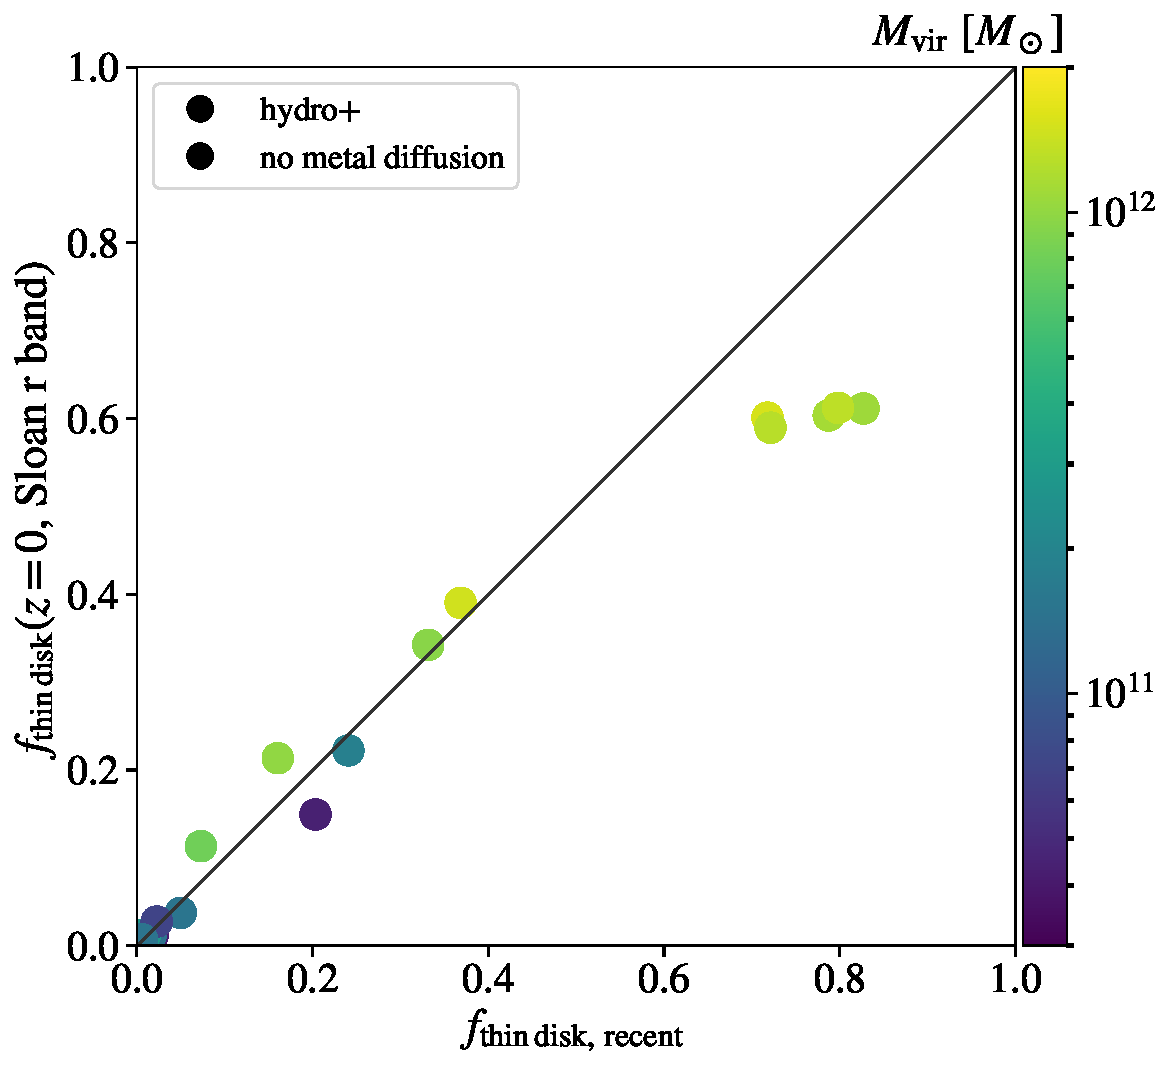
\includegraphics[width=\columnwidth]{figures/prevalence/thin_disk_v_thin_disk.pdf}
    \caption{
    Fraction of recent stars in a thin disc versus Sloan-r-band-weighted thin disc fraction, showing that the thin disc fraction of young stars closely tracks the observationally-motivated luminosity-weighted thin disc fraction.
    }
    \label{f: thin disc v thin disc}
\end{figure}

% Compared to observable-ish thin disc fraction.
Figure~\ref{f: thin disc v thin disc} shows the relationship between the fraction of stars with $j/j_c(E)>0.8$ at $z=0$ ($f_{\rm thin\,disc,\,recent}$) and the same fraction of stars weighted by their Sloan $r$ band luminosity-weighted.
The thin disc metric used throughout our analysis, $f_{\rm thin\,disc,\,recent}$ is closely related to the observationally-motivated luminosity-weighted thin disc fraction.

\section{Sample validation}
\label{s: appendix-sample validation}

% SAMPLE VALIDATION -- TACC
\begin{figure}
    \centering
    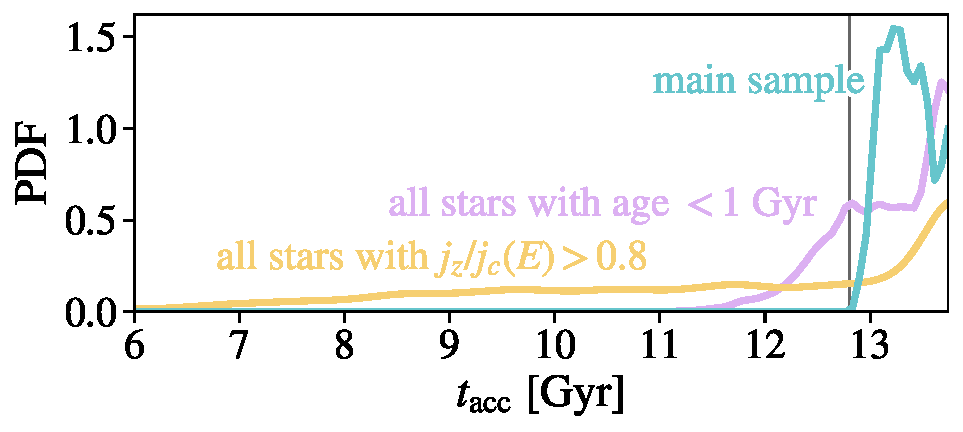
\includegraphics[width=\columnwidth]{figures/selected_to_all_comparison/tacc_m12i_md.pdf}
    \caption{
    Time of accretion for the main sample (green) of 37,189 particles in \texttt{m12i} that are in the CGM at 1 Gyr prior to $z=0$ and in the galaxy at $z=0$, compared to time of accretion for all recent star formation (purple) and all thin disk stars (yellow).
    Time plotted is age of the universe at which gas accreted, with the grey vertical line marking 1 Gyr prior to $z=0$.
    The accretion time of our main sample is representative of the epoch at which accretion occurs for all recent star formation, and overlaps with the accretion times at which \textit{all} thin disk formation peaks.
    }
    \label{f: sample validation -- tacc}
\end{figure}

% SAMPLE VALIDATION - SPATIAL
\begin{figure}
    \centering
    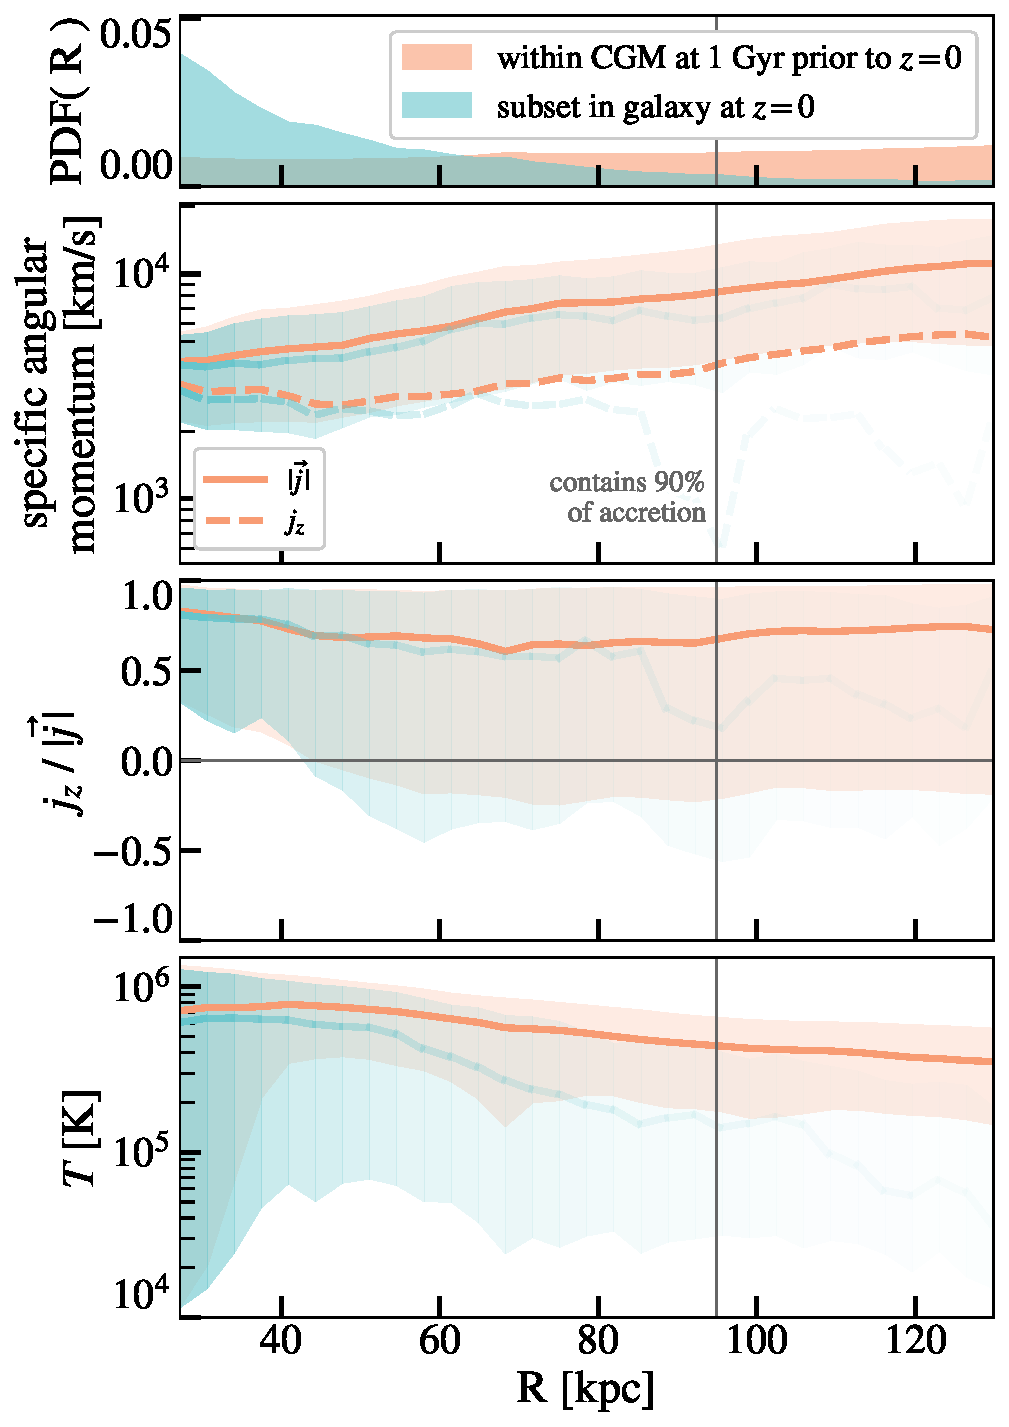
\includegraphics[width=\columnwidth]{figures/selected_to_all_comparison/selected_to_all_comparison_m12i_md.pdf}
    \caption{
    \textbf{Topmost panel:}
    Radial distribution of gas in the CGM of \textit{m12i} at 1 Gyr prior to $z=0$, comparing all gas (orange) to the subset found in the galaxy at $z=0$ (green).
    The main sample preferentially probes the inner CGM, which is capable of accreting prior to $z=0$.
    \textbf{Bottom panels:}
    From top to bottom, specific angular momentum, angular momentum alignment, and temperature for accreted gas and gas at the same radius.
    Solid line shows the median, and the filled regions cover the 16th to 84th percentiles.
    Opacity (darkness) of the accreted gas distribution scales with sample mass fraction found at that radius.
    Gas that accretes by $z=0$ (the main sample) does not have different angular momentum content or alignment compared to gas at the same radii.
    The median temperature is consistent between the main sample and all gas out to 50 kpc, containing the majority of the accreted gas, but our tracked sample preferentially selects mildly cooler gas.
    }
    \label{f: sample validation -- spatial}
\end{figure}

% Intro
Our main sample of tracked particles for each simulation, detailed in \S\ref{s: methods -- analysis}, was selected with the aim of following with high mass resolution the history of interacting accreting gas.
This allows us to calculate, for example, the extent to which heating and cooling balance (Fig.~\ref{f: before and after B}, panel D).
In this appendix we check the extent to which our sample is representative of the accretion that fuels all recent star formation, and the accretion that fuels all thin disk star formation, and gas at the same radius in the halo.
We use single simulation, \texttt{m12i}, as a test case.

% Accretion times
Fig.~\ref{f: sample validation -- tacc} shows the age of the universe at which resolution elements in our main sample accrete onto the main galaxy, compared to the time at which gas accretes onto the galaxy for all recently-formed stars and all thin-disk stars.
To calculate the accretion time ($t_{\rm acc}$) distribution for all recently-formed stars and all thin-disk stars we tracked the history of $10^5$ randomly-selected star particles that formed within the last Gyr and had circularity $(j_z/j_c(E))\vert_{z=0} > 0.8$ respectively.
Particles may accrete onto the galaxy several times (recycling; e.g. \citealt{Angles-Alcazar2017}).
For our main sample we chose the time of accretion as the first time the gas accretes after being located in the CGM at 1 Gyr prior to $z=0$, consistent with our analysis in the main text.
For the two alternative samples we chose the time of accretion as the last time the gas accretes onto the galaxy prior to forming a star.
The accretion time distribution for the main sample and the sample probing all recently-formed stars overlaps strongly, and also overlaps with the time at which formation of thin disk stars peaks.
The degree of overlap we see in the $t_{\rm acc}$ distributions between our sample and the sample probing all recent star formation validates the stronge correlation between properties of our sample and the fraction of recently formed stars found in a thin disk (Figs~\ref{f: prevalence} and~\ref{f: prevalence - angular momentum}).

% Spatial
Fig.~\ref{f: sample validation -- spatial} shows the properties of our main sample compared to gas at the same radius, which allows us to assess if accreting gas is representative of all CGM gas at the same redshift.
From Fig.~\ref{f: sample validation -- spatial} we learn that (a) gas that accretes within a fixed time of 1 Gyr is limited to $r \lesssim 100$ kpc;
(b) on a per-particle basis the specific angular momentum magnitude, the z-direction specific angular momentum, and the ratio of the two are very similar between all gas and accreted gas;
and (c) the temperature of accreted gas and all gas at the same radius is consistent, but some cooler, less-pressure-supported gas at larger radii can accrete onto the galaxy.
These results are consistent with the temperature distributions for accreting gas vs gas that remains in the CGM for $>3$ Gyr~\citep{Hafen2020}.

\section{Accretion onto haloes absent thin discs}
\label{s: appendix-low mass}

% COUNTEREXAMPLE
\begin{figure*}
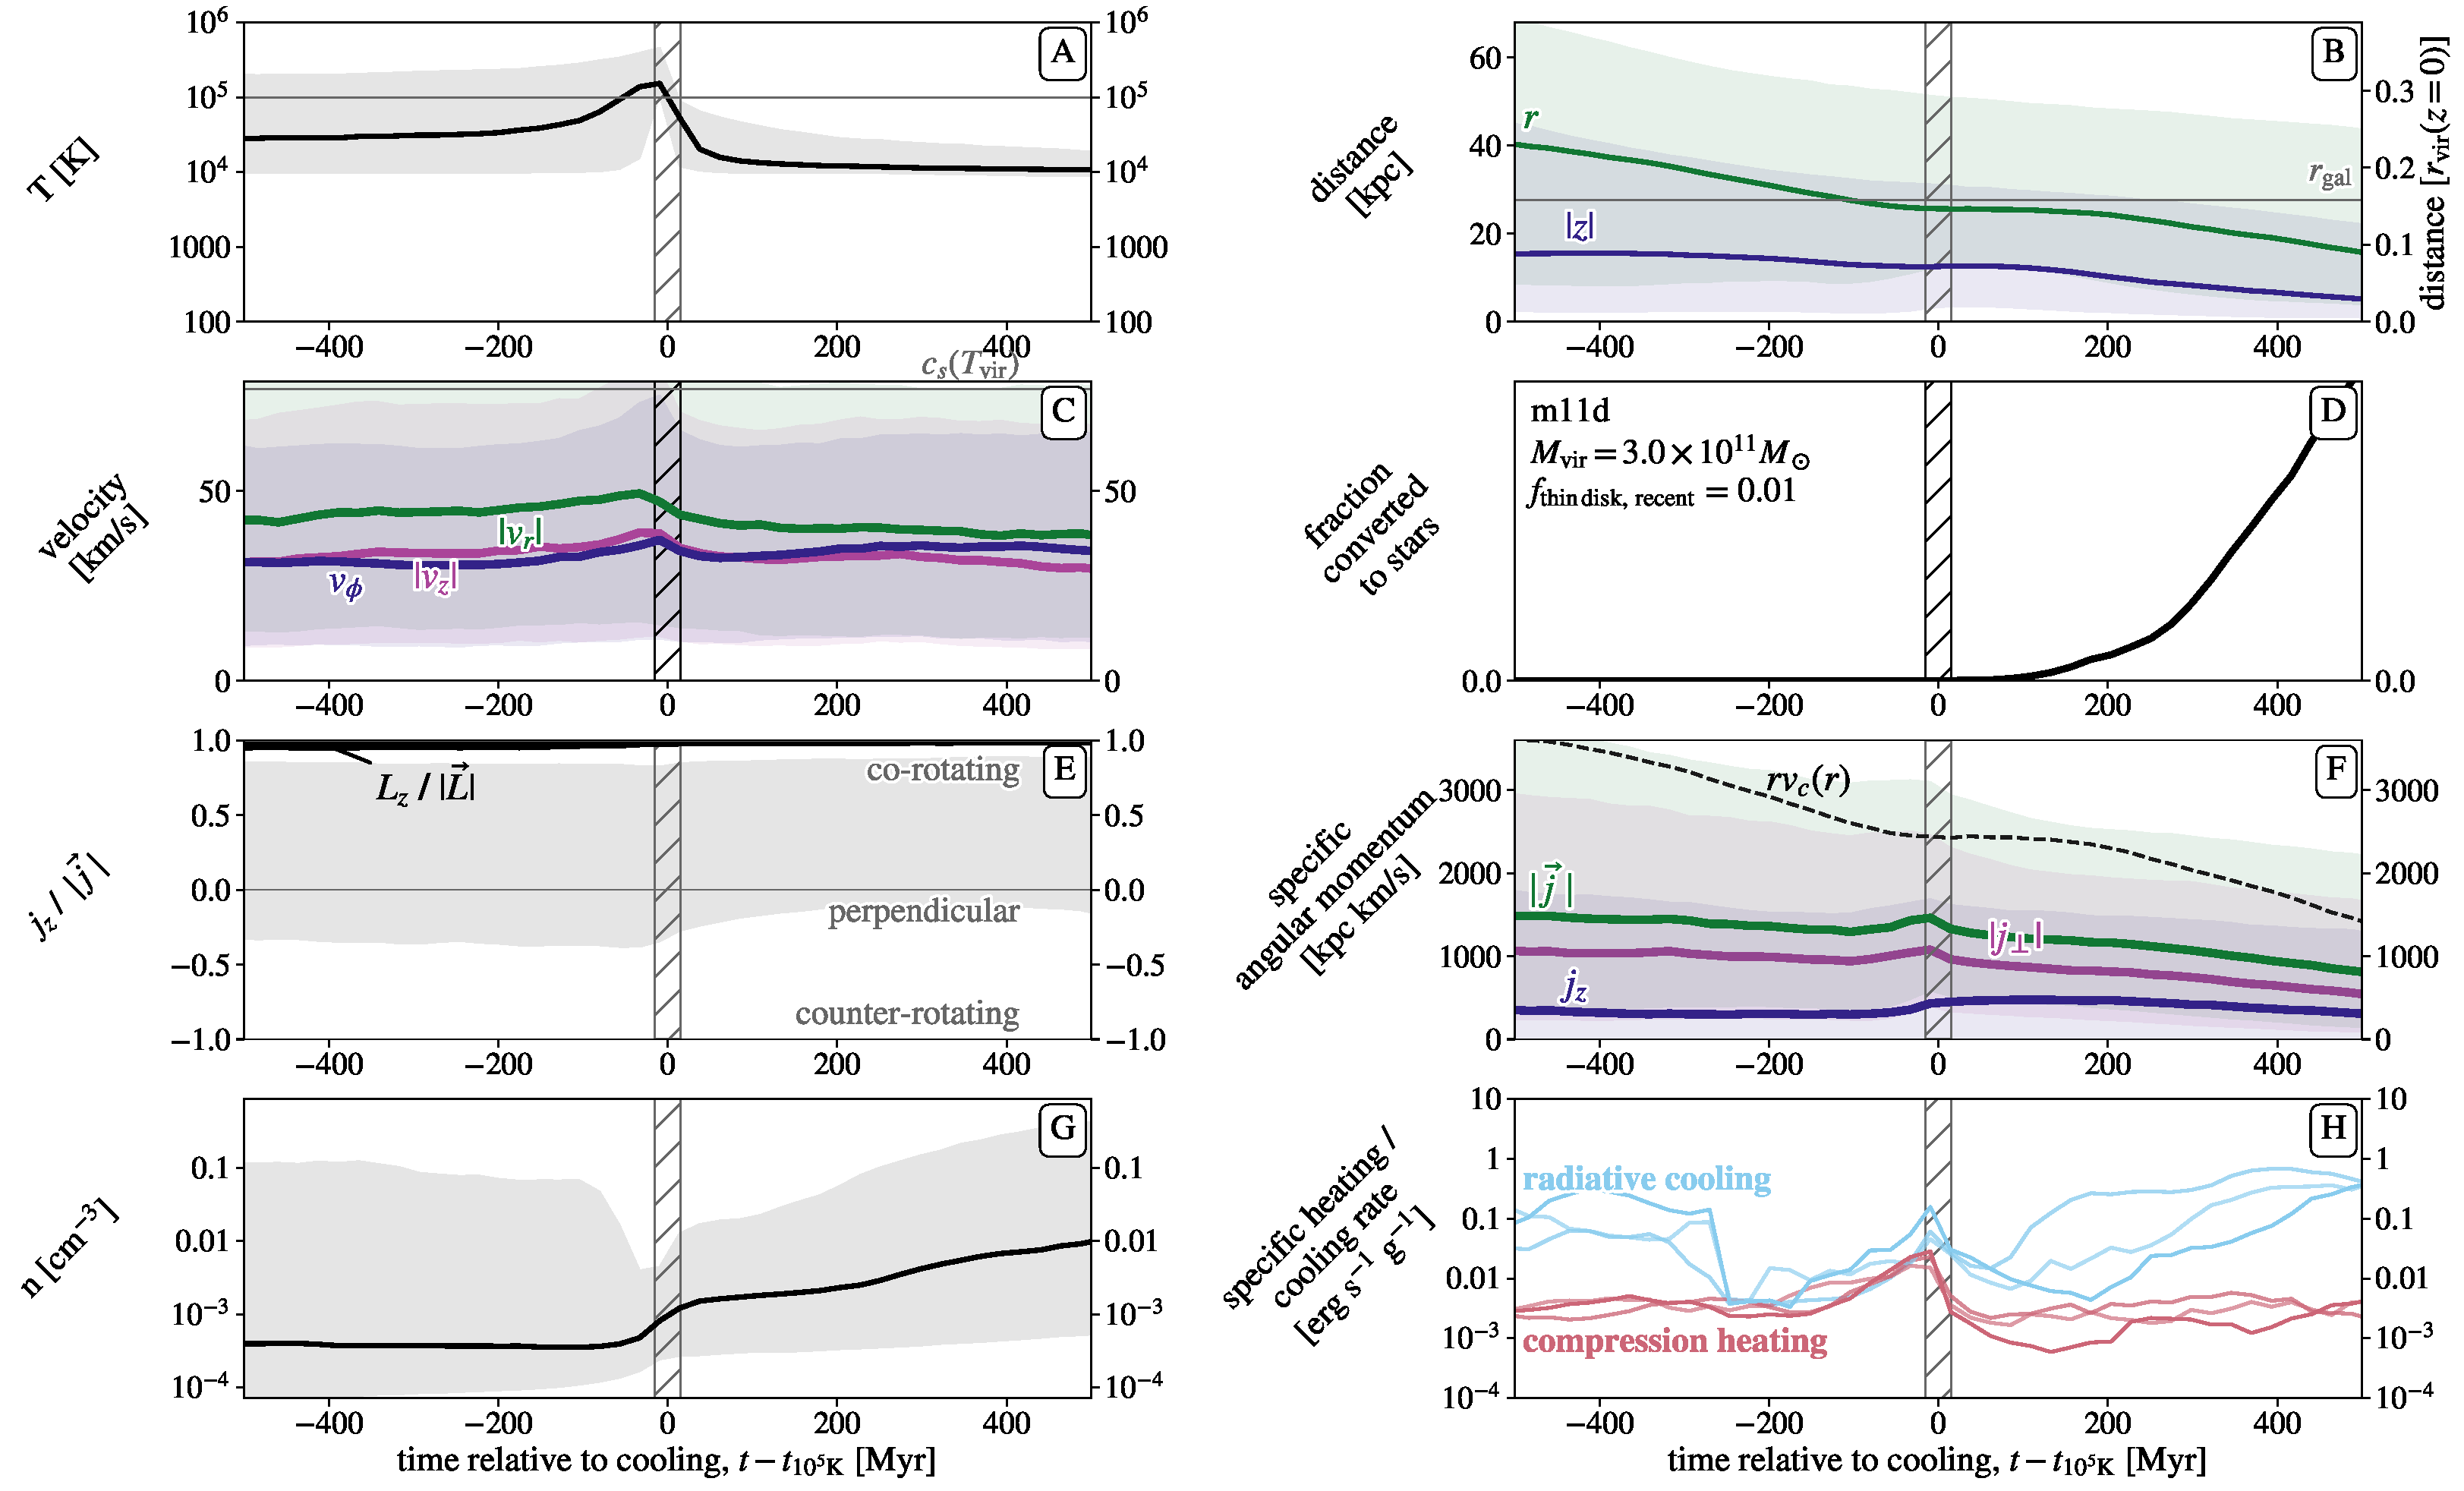
\includegraphics[width=\textwidth]{figures/before_and_after/before_and_after_allone_m11d_md.pdf}
\caption{
Temperature and geometry of gas accreting onto a representative $z\sim0$ galaxy in FIRE that does \textit{not} form a thin disc, versus time relative to the final cooling time ($t - \tcools$).
This figure should be compared with Figs~\ref{f: before and after A} and~\ref{f: before and after B}.
In each panel solid lines and shaded regions mark the medians and 16th to 84th percentile ranges of all particles accreted within 1 Gyr prior to $z=0$.
\textbf{A:} Temperature.
The final cooling tends to occur shortly after the gas is heated beyond $T=10^5$ K.
\textbf{B:} 3D distance from halo center.
\textbf{C:} Absolute height from the disc plane.
\textbf{D:} Velocity components of accretion (colored lines and band), relative to circular velocity at the median radius (dash-dotted line).
\textbf{E:} Fraction of gas converted into stars.
Star formation proceeds shortly after cooling, well before gas orients into a disc.
\textbf{F:} The ratio of $j_z / \vert \vec j \vert$.
The solid line shows this ratio for the total angular momentum of all accreted particles.
The coherence of the gas does not change before/after cooling.
\textbf{G:} The magnitude of the specific angular momentum of particles ($\vert\vec{j}\vert$, green) and the component of angular momentum aligned with the galaxy disc ($j_z$; purple).
The dashed line shows the angular momentum necessary for rotational support.
Rotational support occurs $\gtrsim 300$ Myr after $\tcools$, at which time inward movement stalls and gas velocity decreases.
\textbf{H:} Baryon number density.
\textbf{I:} Energy loss from radiative cooling (blue) and heating from $PdV$ work on the gas particles (red).
Radiative cooling exceeds compression heating with the exception of when the gas is heated, shortly before cooling.
}
\label{f: counterexample}
\end{figure*}

Figure~\ref{f: counterexample} shows characteristic accretion onto a halo with a small (in this case nearly zero) thin disc fraction.
Such haloes do not show the features of rotating cooling flows, as also seen in Figures~\ref{f: prevalence} and~\ref{f: prevalence - angular momentum}.

\section{Accretion onto other MW-mass haloes}
\label{s: appendix-other m12s}

% M12B
\begin{figure*}
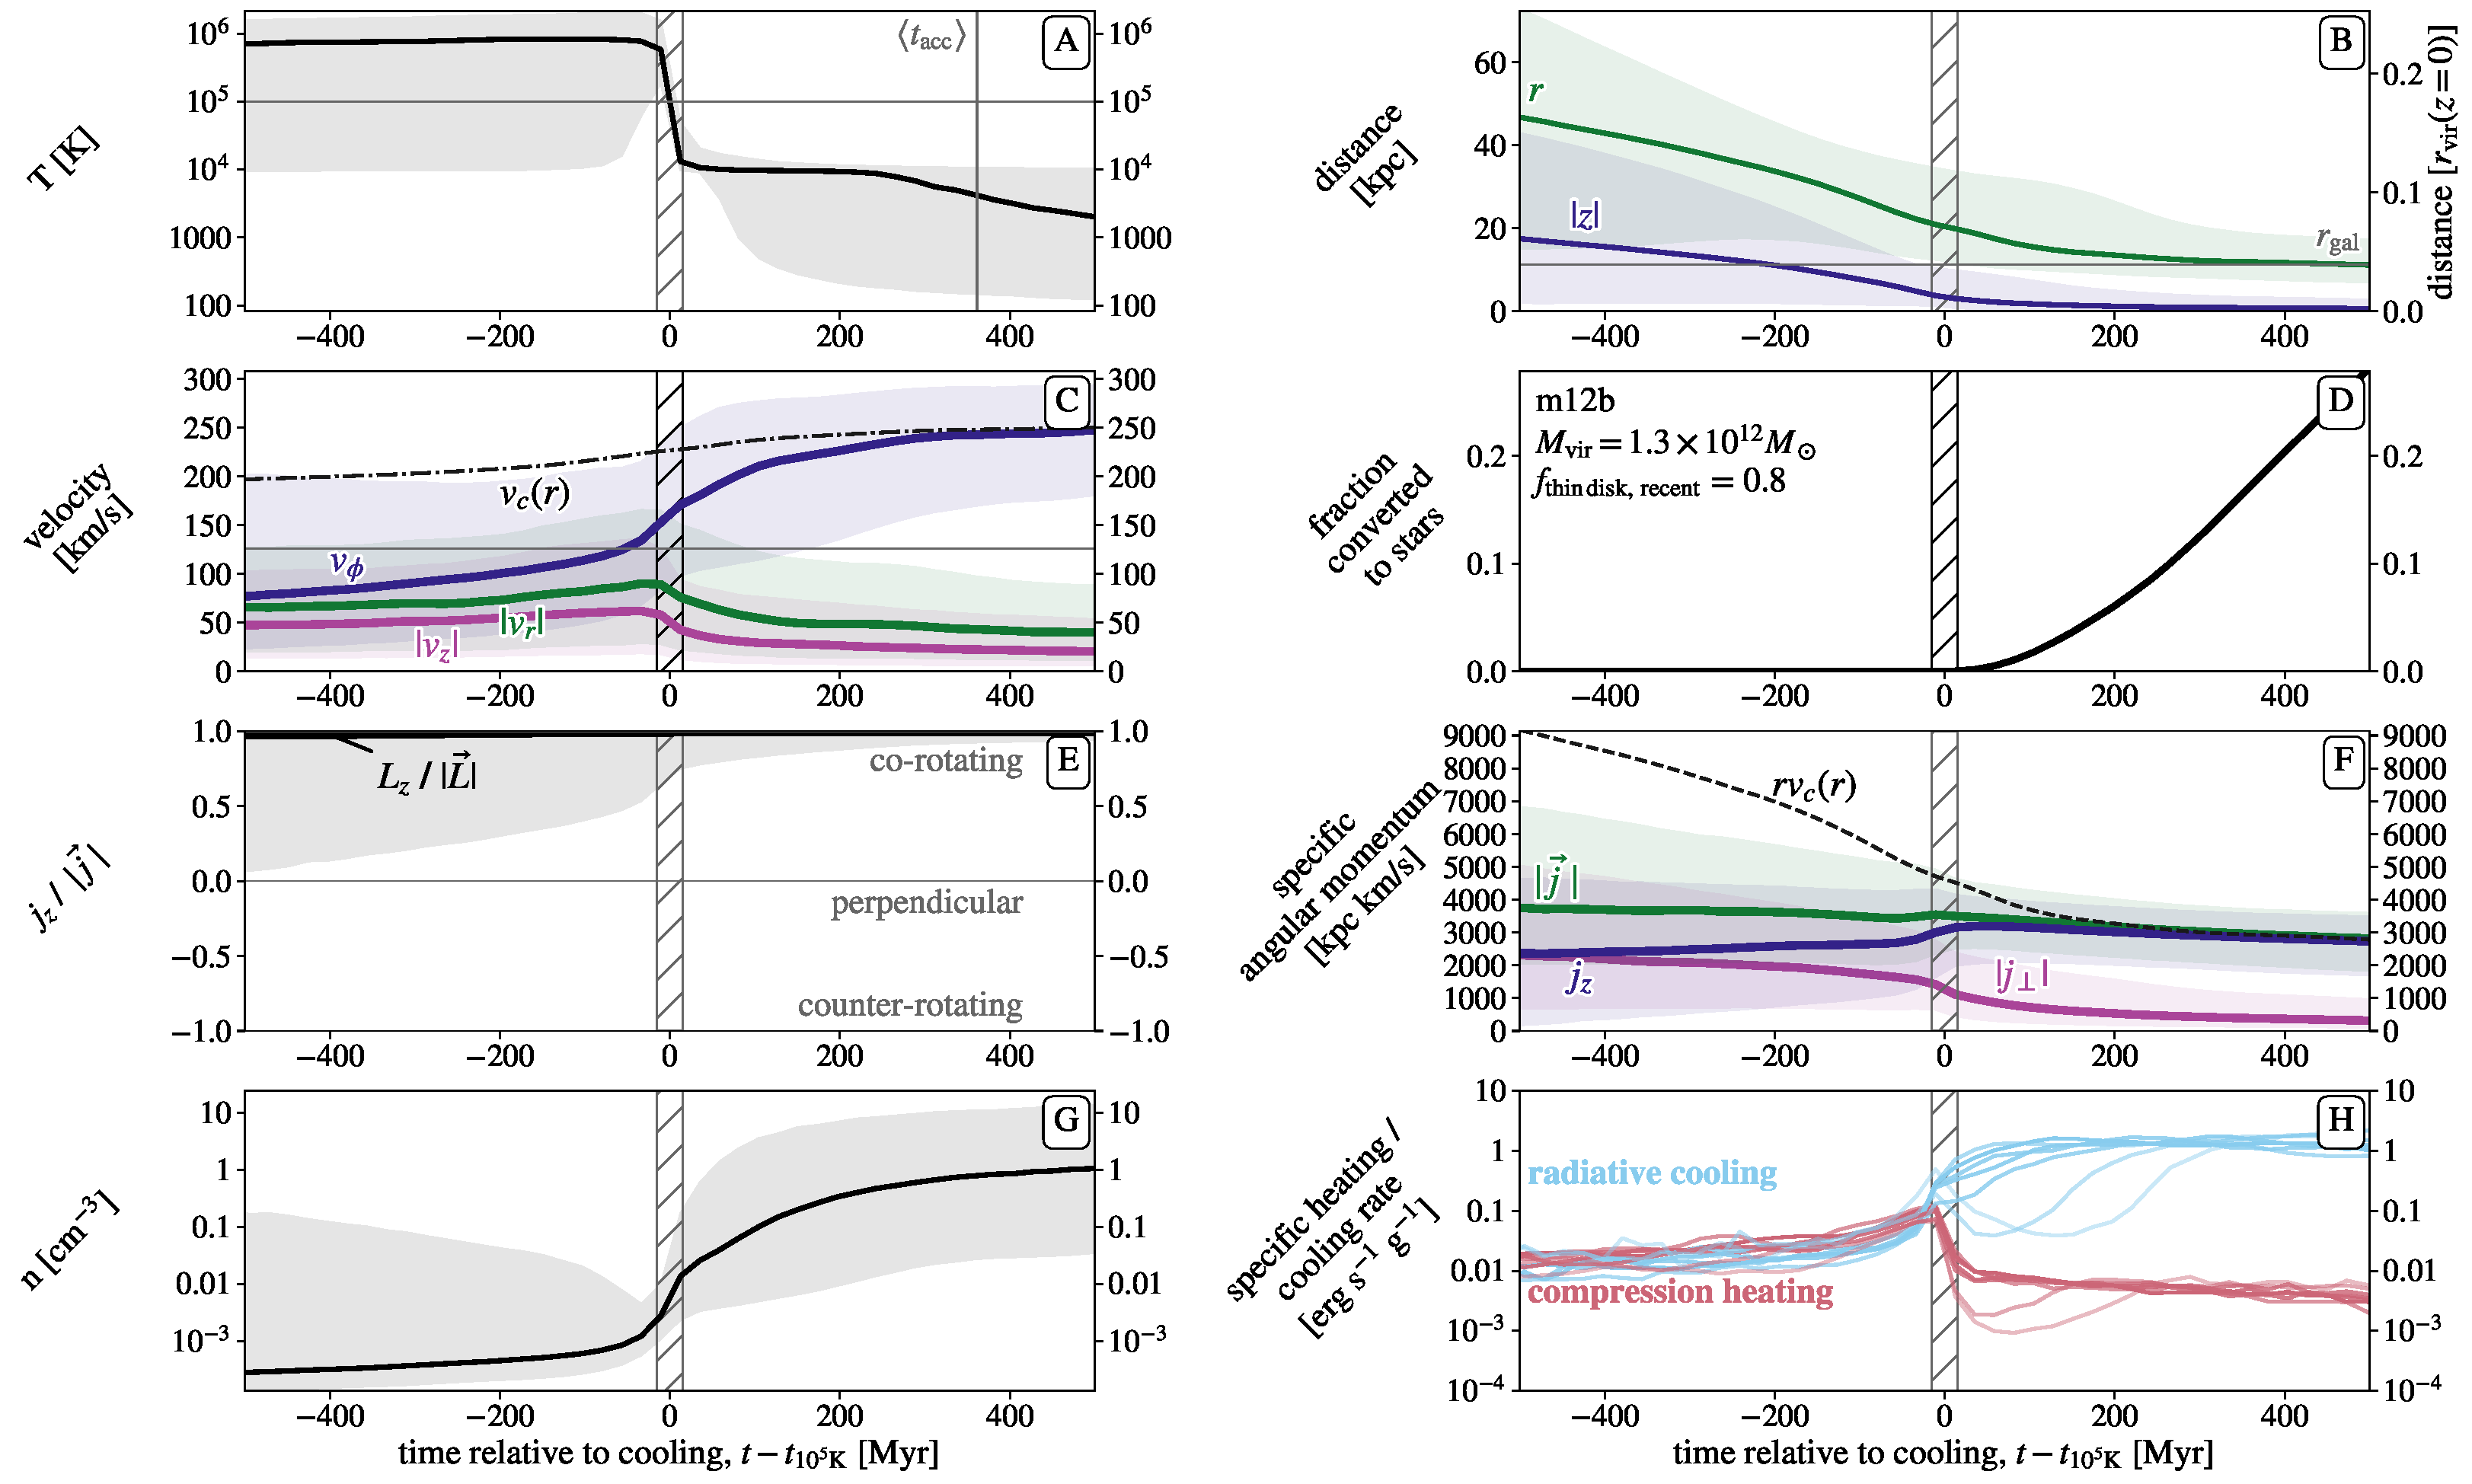
\includegraphics[width=\textwidth]{figures/before_and_after/before_and_after_allone_m12b_md.pdf}
\caption{
Same as Figure~\ref{f: counterexample}, but for a MW-mass halo with a thin disc, \texttt{m12b}.
}
\label{f: before and after m12b}
\end{figure*}

% M12C
\begin{figure*}
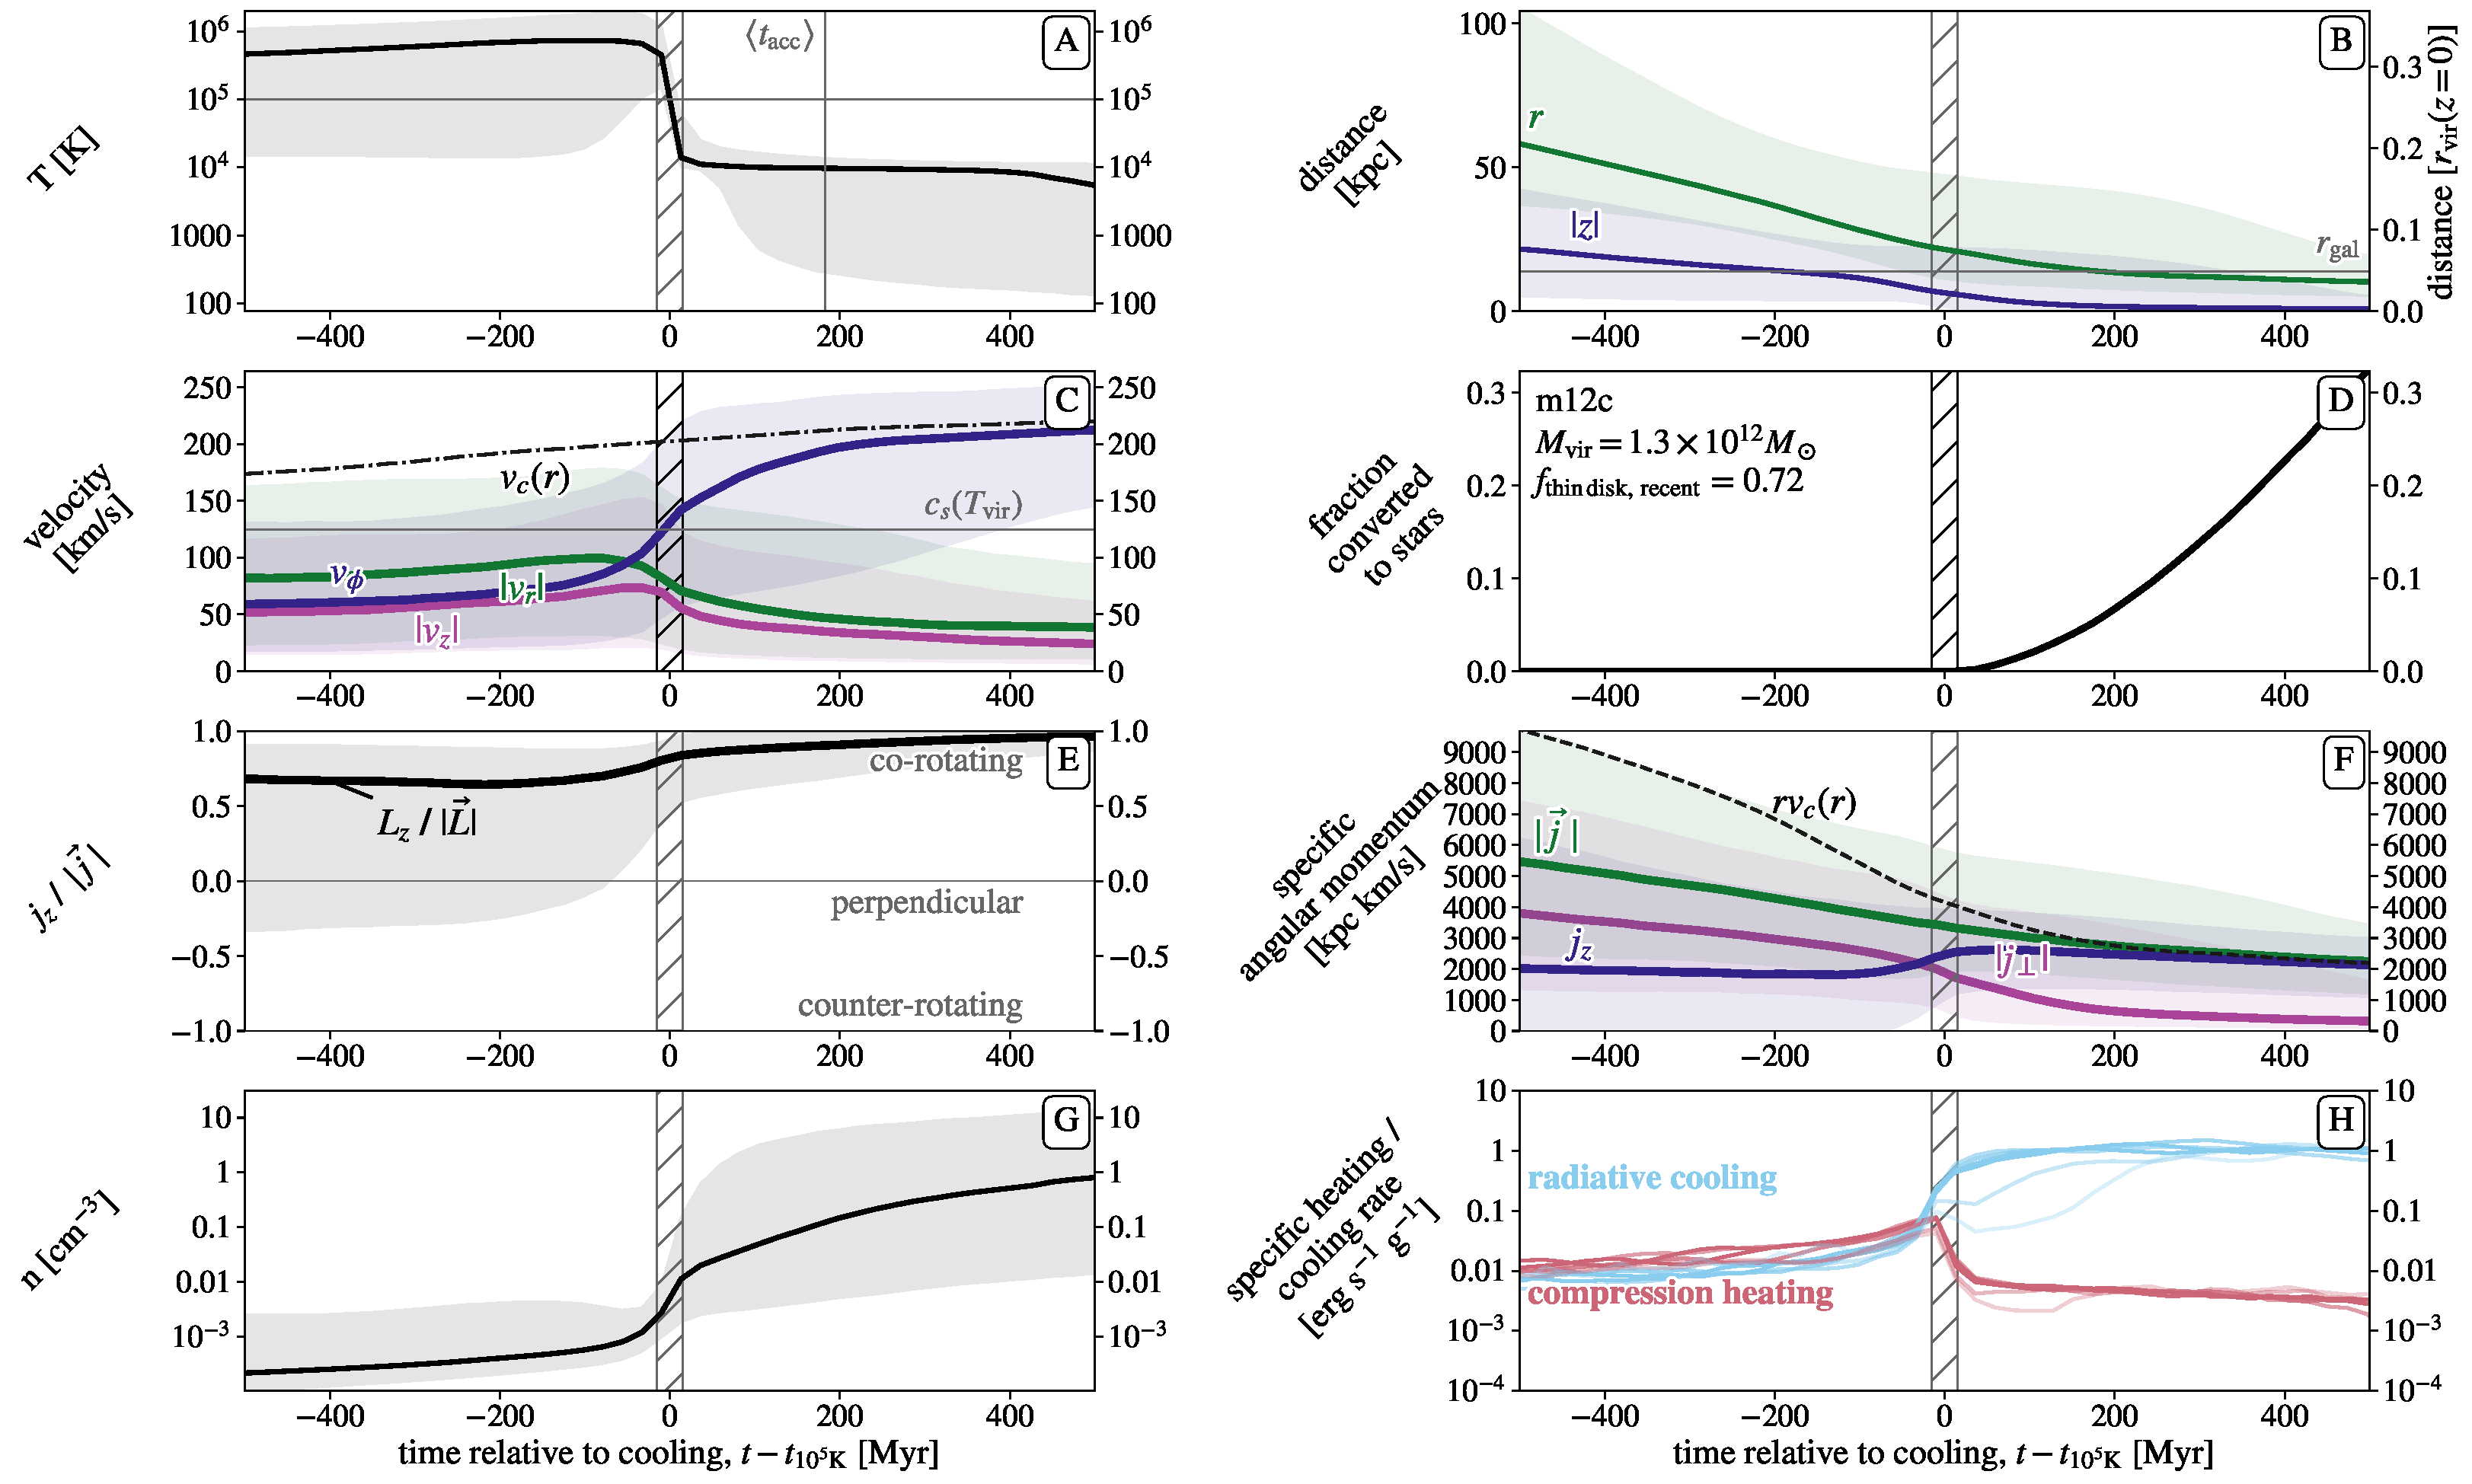
\includegraphics[width=\textwidth]{figures/before_and_after/before_and_after_allone_m12c_md.pdf}
\caption{
Same as Figure~\ref{f: counterexample}, but for another MW-mass halo with a thin disc, \texttt{m12c}.
}
\label{f: before and after m12c}
\end{figure*}

Figures~\ref{f: before and after m12b} and~\ref{f: before and after m12c} show the combined equivalent of Figures~\ref{f: before and after A} and~\ref{f: before and after B} for two other Milky Way-mass haloes.
The behavior is qualitatively very similar to each other and \texttt{m12i}.
This is summarized for additional simulations in Figures~\ref{f: prevalence} and~\ref{f: prevalence - angular momentum}.

\section{Accretion in cosmic ray-dominated haloes}
\label{s: appendix-crs}

% M12I_CR
\begin{figure*}
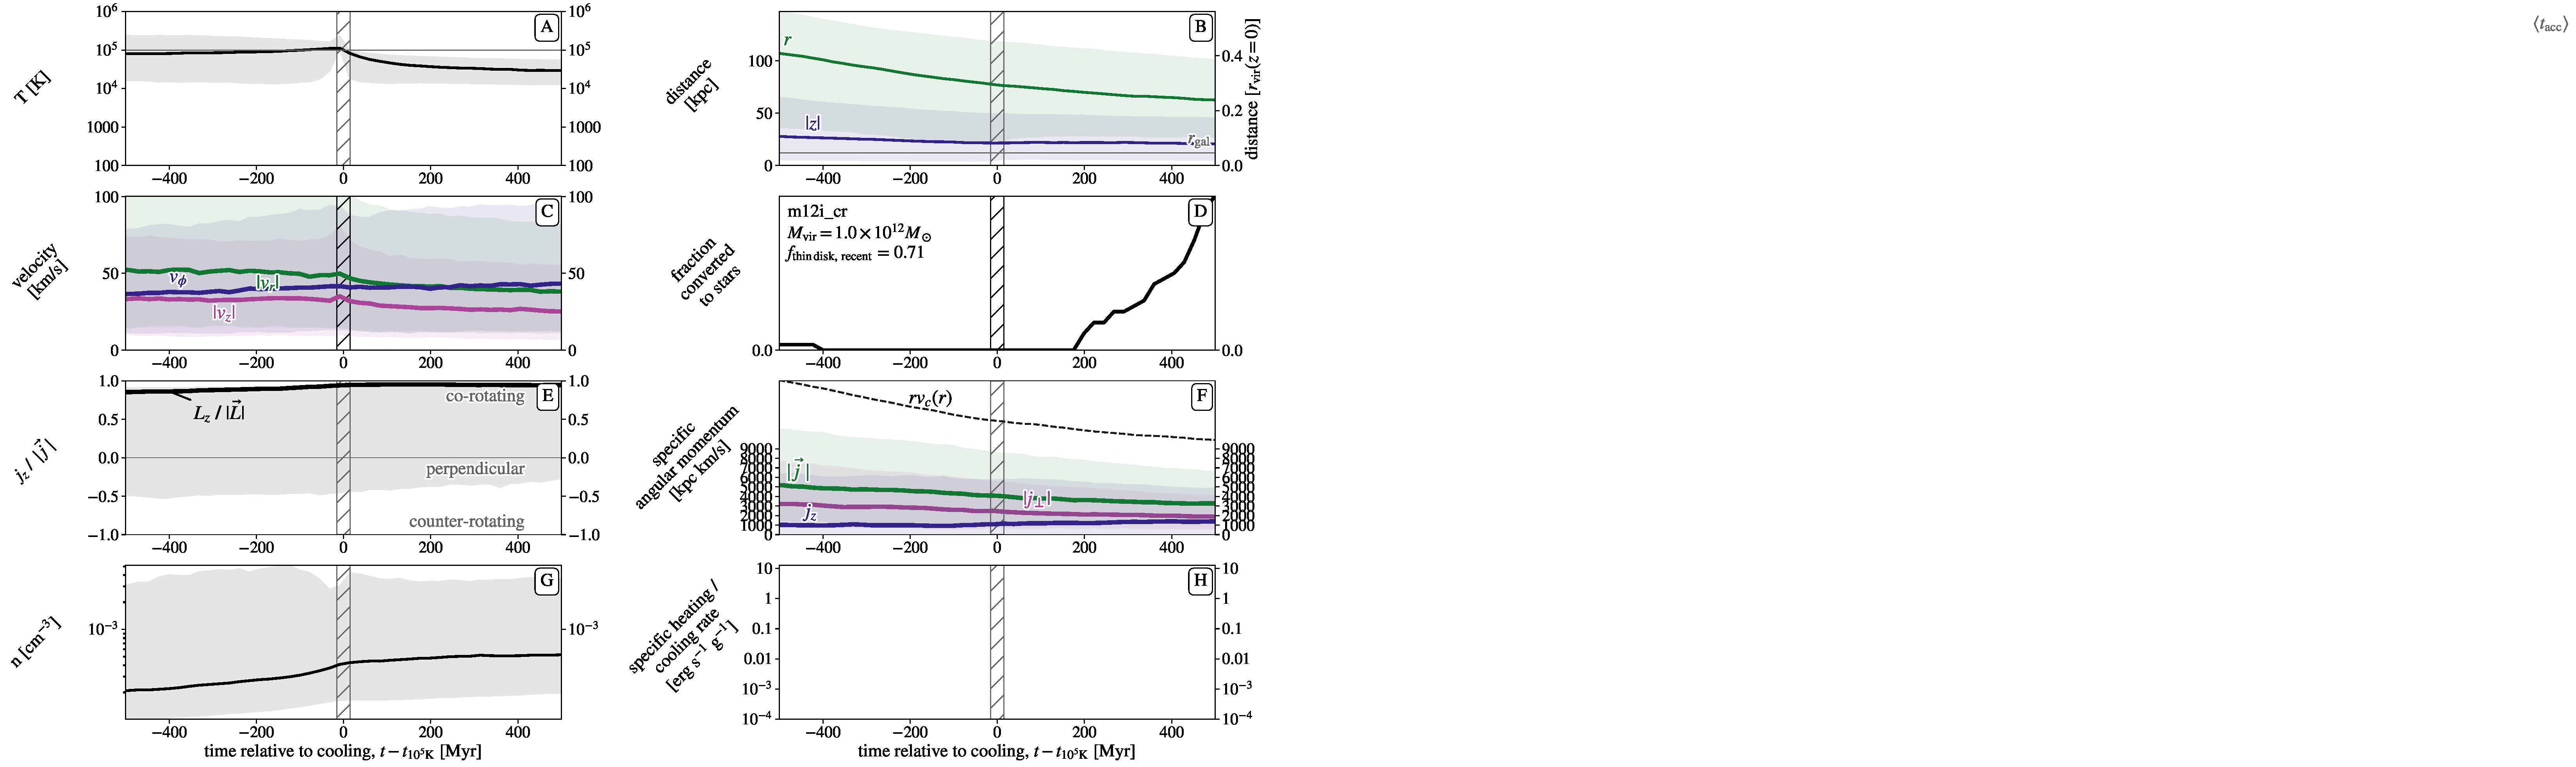
\includegraphics[width=\textwidth]{figures/before_and_after/before_and_after_allone_m12i_cr.pdf}
\caption{
Same as Figure~\ref{f: counterexample}, but for a cosmic ray-dominated MW-mass halo, \texttt{m12i\_cr}.
The accretion in cosmic ray-dominated haloes is qualitatively similar to rotating cooling flows.
The exceptions are the temperature (panel A) and the energy balance (panel B): nonthermal support from cosmic rays (CRs) produces a $T\sim 10^4$ K, diffuse halo absent cooling flows.
As with rotating cooling flows accreting gas in this halo becomes coherently aligned \textit{prior to accretion}, a key mechanism that enables thin disc formation.
}
\label{f: before and after m12i cr}
\end{figure*}

Figure~\ref{f: before and after m12i cr} shows the combined equivalent of Figures~\ref{f: before and after A} and~\ref{f: before and after B} for the same halo, but with an implementation of cosmic ray feedback~\cite{Chan2019, Hopkins2020a}.
Note that we center the trajectories on the time of first accretion instead of $\tcools$ because in CR-dominated haloes much of the gas is never heated beyond $T = 10^5$ K.
This does not significantly affect the result, as accretion is largely concurrent with cooling in the haloes without CRs.
This halo forms a thin disc ($f_{\rm thin\,disc,\,recent}=0.71$, which we argue may be a general feature of rotating subsonic flows~(\S\ref{s: why CFs thin discs}, \S\ref{s: crs}).
Note that in panel B we only plot radiative cooling and compression heating, i.e. we do not show photoionization heating, which is responsible for offsetting the radiative cooling and maintaining a temperature of $T \sim 10^4$ K.

\section{Instantaneous mass flow}
\label{s: appendix-mass flow}

% HOT IN HALO
\begin{figure*}
    \centering
    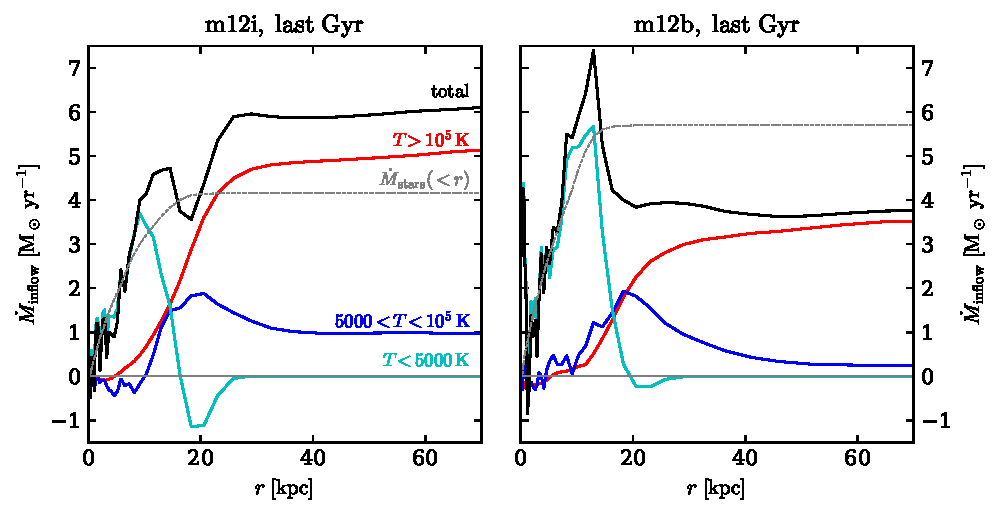
\includegraphics{figures/Mdot.pdf}
    \caption{
    Average mass inflow rate over the course of one Gyr prior to $z=0$ in the same haloes as in Figure~\ref{f: stars}, by gas temperature.
    The galaxy radius $r_{\rm gal}=4 r_{\star,0.5}$ and fraction of stars in a thin disc are marked in the panels. 
    Hot accretion ($T>10^5$ K) dominates the mass inflow onto thin-disc galaxies at $r \gtrsim r_{\rm gal} \sim 10-20$ kpc.
    Cold accretion ($T<10^5$ K) dominates within the galaxy in thin disc galaxies, and in the halo of the lower-mass irregular galaxy shown in the bottom-right panel.
    }
    \label{f: Mdot}
\end{figure*}

In this section we analyse if inflow is dominated by hot or cold gas, which allows us to distinguish a hot inflow from the accretion of cool clouds (formed, e.g., via instabilities).
Figure~\ref{f: Mdot} shows the mass inflow rate versus radius for hot gas (red curves; $T>10^5$ K) and for cool gas (blue curves; $T < 10^5\,{\rm K}$),  for the four simulations shown in Fig.~\ref{f: stars}. 
We calculate the mass inflow rate at a given radius as
\begin{equation}
     \Mdot(r) = \frac{\int_{\rm shell} v_r dm}{\Delta r} = \frac{M_{\rm shell}}{\Delta r} \langle v_r\rangle_{\rm mass\, weighted}
     \label{e: Mdot}
\end{equation}
where $\Delta r=0.05\,{\rm dex}$ is the shell thickness, and the integration is done on all particles with centers within the shell which satisfy the appropriate temperature cut. 

% Consequences
In the three MW-mass galaxies with a large thin disc fraction, at halo scales of $r>20$ kpc the inflow is dominated by hot gas, where in \texttt{m12i} and \texttt{m12b} $\Mdot$ of the hot gas is larger by a factor of $\gtrsim 4\times$ than that of cool gas.
The greater mass flux of hot gas indicates that the dominant form of accretion is an inflowing hot phase, rather than cold streams or cool clouds precipitating from the hot phase.
In contrast, in the lower mass galaxy shown in the bottom right the inflow is dominated by cool gas, while the hot gas is outflowing out to $\approx50$ kpc.
Fig.~\ref{f: Mdot} also shows that the inflow rate of hot gas in the MW-mass galaxies drops within $r_{\rm gal}$, reflecting the cooling of the hot inflow at the galaxy-halo interface, as shown in \S\ref{s: characteristics -- cools}.

\section{Notes on individual galaxies}

\label{s: appendix-individual}

% Presence of a rotating cooling flow for intermediate cases
The haloes with $0.1 \lesssim f_{\rm thin\,disc,\,recent} < 0.5$ have varying levels of circularized cooling flow accretion.
Four of these six haloes, \texttt{m12z}, \texttt{m12r}, \texttt{m12w}, and \texttt{m12m}, have $M_{\rm vir} \sim 10^{12} M_\odot$.
\texttt{m12z} has a chaotic halo with a number of ongoing mergers.
\texttt{m12r} has some ongoing thin disc formation, but is undergoing a major merger during the last Gyr that dominates the accreting gas supply and disrupts the galaxy structure.
This merger is relatively well-aligned with the disc, with $f_{\rm aligned} \approx 0.3-0.4$, and the aligned mass fraction does not change significantly as the gas cools past $\tcools$.
\texttt{m12w} is a galaxy with its inner CGM is only just virializing at $z=0$~\citep{Yu2021}, and the majority of the gas accretes with angular momentum perpendicular to the galaxy angular momentum.
Of these four the one with the highest thin disc fraction, \texttt{m12m}, is galaxy undergoing significant rotating cooling flow accretion, but absent a high thin disc fraction.
Visual inspection reveals that \texttt{m12m} has a prominent stellar bar.
\texttt{m12m} may be evidence that if rotating cooling flows are a condition for disc formation, they are a necessary-but-not-sufficient condition (\S\ref{s: why CFs thin discs}).
\texttt{m12m} is one of the few MW-mass haloes that does not include metal diffusion, which may play a role in its morphology.
The $M_{\rm vir} \sim 10^{11} M_\odot$ haloes are \texttt{m11h} and \texttt{m11b} --- galaxies that are beginning to form discs despite their lower virial mass.
Much of their accretion is still isotropic, but alignment increases mildly post-cooling.

%%%%%%%%%%%%%%%%%%%%%%%%%%%%%%%%%%%%%%%%%%%%%%%%%%

% Don't change these lines
\bsp	% typesetting comment
\label{lastpage}
\end{document}

% End of mnras_template.tex
 